\documentclass[a4paper,12pt,twoside,openright]{book}

\usepackage[a4paper]{geometry}
\usepackage[T1]    {fontenc }% Allow accented output charachters
\usepackage[utf8]  {inputenc}% Allow accented input charachters 
\usepackage        {lmodern }% Modern output font	
\def\magyarOptions{suggestions=no}
\usepackage[magyar]{babel}	   % Set document language to use
\usepackage		 {amsmath}%Math mode additions
\usepackage		 {amsfonts}
\usepackage{MnSymbol}
\usepackage{amsthm}
\usepackage		 {floatrow}% Append additional information to images (source)
\usepackage		{mathtools}
\usepackage[pdftex]{graphicx}% Adds the ability to include images 
\usepackage		 {xcolor   }% Colors are fun :)
\usepackage        {colortbl}% Named even more. 
\usepackage        {url     }% Makes urls clickable 
\usepackage		{array}
\usepackage		 {tikz	  }% Latex drawn figures
\usetikzlibrary{shapes,calc,positioning}
\usepackage		{wrapfig}
\usepackage{fixltx2e}
\usepackage		{relsize}
\usetikzlibrary	 {matrix  }
\usepackage		{textcomp}
\usepackage        {scalefnt }% Scale the latex drawn figure elements
\usepackage[pdf]{pstricks}
\usepackage{subfigure}
\usepackage{enumerate}

\usepackage{titlesec}
\newcommand{\sectionbreak}{\clearpage}

% The csquotes should be used with bable to help with the references formating 
\usepackage[style=english]{csquotes} 
% Biblatex
\usepackage[style=ieee,
backend=biber,babel=other*, language=english, sorting=none,
backref=false]{biblatex} \DeclareSourcemap{ % Unfortunetly the
% bibtex currently knows of online type, not webpage. For now just map it.
  \maps[datatype=bibtex]{
    \map{
      \step[typesource=webpage, typetarget=online]
    }
  }
}

\newcommand*\circled[1]{\tikz[baseline=(char.base)]{
            \node[shape=circle,draw,inner sep=1pt] (char) {#1};}}

% Smiley commands
\newcommand{\smiley}{\tikz[baseline=-0.75ex,ColorGreyish]{
    \draw circle (2mm);
\node[fill,circle,inner sep=0.5pt] (left eye) at (135:0.8mm) {};
\node[fill,circle,inner sep=0.5pt] (right eye) at (45:0.8mm) {}; \draw
(-145:0.9mm) arc (-120:-60:1.5mm);
    }
}

\newcommand{\frownie}{\tikz[baseline=-0.75ex,orange]{
    \draw circle (2mm);
\node[fill,circle,inner sep=0.5pt] (left eye) at (135:0.8mm) {};
\node[fill,circle,inner sep=0.5pt] (right eye) at (45:0.8mm) {}; \draw
(-145:0.9mm) arc (120:60:1.5mm);
    }
}

\newcommand{\neutranie}{\tikz[baseline=-0.75ex,black]{
    \draw circle (2mm);
\node[fill,circle,inner sep=0.5pt] (left eye) at (135:0.8mm) {};
\node[fill,circle,inner sep=0.5pt] (right eye) at (45:0.8mm) {}; \draw
(-135:0.9mm) -- (-45:0.9mm);
    }
}
% Background highlight color used for the source code and the tables
\definecolor{bgSrc}{rgb}{0.95,0.95,0.95}
\colorlet{ColorGreyish}{black!10}

\usepackage[unicode]{hyperref}% - Add links between the doc
\usepackage[all]{hypcap}   %Let the links point above figures and not below
\usepackage[numbered,
			  open, 
			  openlevel=2,
			  atend]{bookmark}% - We want numbers

\usepackage{fancyhdr}
\setlength{\headheight}{30pt}

\pagestyle{fancy}
\renewcommand{\chaptermark}[1]{ \markboth{#1}{} }
\renewcommand{\sectionmark}[1]{ \markright{#1}{} }

\fancyhf{}
\fancyhead[LE,RO]{\thepage}
\fancyhead[RE]{\textit{ \nouppercase{\leftmark}} }
\fancyhead[LO]{\textit{ \nouppercase{\rightmark}} }

\fancypagestyle{plain}{ %
  \fancyhf{} % remove everything
  \renewcommand{\headrulewidth}{0pt} % remove lines as well
  \renewcommand{\footrulewidth}{0pt}
}

\usepackage{changepage,ifthen}
\newcommand\skiptooddpage{%
   \checkoddpage
   \ifthenelse{\boolean{oddpage}}%
      {\null\clearpage \null \clearpage}%
      {\null\clearpage}%
}

\usepackage{chngcntr}
\counterwithout{section}{chapter}
\counterwithout{footnote}{chapter}
\counterwithout{figure}{chapter}

\usepackage{tocbibind}

\begin{document}

% A címlap
% !TeX encoding = UTF-8 
% !TeX spellcheck =hu_HU
\hypersetup{pageanchor=false}
\begin{titlepage}
\newcommand{\HRule}{\rule{\linewidth}{0.5mm}}
\begin{center}


\includegraphics[width=0.5\textwidth]{./kepek/Budapest-logo.jpg}\\
\textsc{Budapest Műszaki és Gazdaságtudományi Egyetem}\\
\textsc{Villamosmérnöki és Informatikai Kar}\\
\textsc{Számítástudományi és Információelméleti Tanszék}\\[1.5cm]
\textsc{Rendszeroptimalizálás -- BMEVISZM117}\\[0.5cm]

% Title
\HRule \\[0.4cm]
{ \huge \bfseries Rendszeroptimalizálás}\\[0.4cm]
{Vizsga tételsor jegyzet}

\HRule \\[1.5cm]

% Author and supervisor
\begin{minipage}{0.4\textwidth}
\begin{flushleft} \large
\emph{Szerző:}\\
\textsc{Gábor} Bernát
\end{flushleft}
\end{minipage}

\vfill
% Bottom of the page
{\large \today}
\end{center}
\end{titlepage}
\hypersetup{pageanchor=false}


\tableofcontents
\chapter{Lineáris programozás}
\hyphenation{Egerváry}
\section{Egerváry algoritmusa, az optimális hozzárendelés problémája}

Az optimális hozzárendelés problémája a következő kérdésre keresi a választ:
hogyan rendelünk egymáshoz két halmaz elemeit valamilyen optimum kritérium
szerint? Ilyen kritériumok lehetnek a maximális párosítás~\footnote{ Párosításnak
nevezünk egy $M$ élhalmazt, ha semelyik két élnek nincs közös pontja (független
él halmaz). Egy párosítás teljes, ha a gráf minden pontját lefedi.}, minimális
idő igény és így tovább. Grafikusan ábrázolva, legyen:

\begin{figure}[ht]
\caption{Egy optimális hozzárendelés probléma}
\label{fig:OptHozProb}
\centering \begin{tikzpicture}[scale=1.7]
  \tikzset{ p/.style={circle,yellow,fill=red,inner sep=0pt,minimum size=0.15cm},
  }
 % the two sets
  \draw (0,0) ellipse (1.2cm and 0.3cm) node [right=2.1cm] {Elvégezendő munka -- $A$};
  \draw (0,1.5) ellipse (1.2cm and 0.3cm) node [right=2.1cm] {Rendelkezésre álló munkások --
  $B$};
  % the dots
  \node[p] (lB) at (-1, 0) {};
  \node[p] (lT) at (+1, 0) {}; 
  \node[p] (lC) at ( 0  , 0) {};
  
  \node[p] (rB) at (-1, 1.5) {}; 
  \node[p] (rT) at (+1, 1.5) {}; 
  \node[p] (rC) at ( 0, 1.5) {};
  
  % the connection between the dots
  \draw[-] (lT) -- (rC); 
  \draw[-] (lC) -- (rC); 
  \draw[-] (lB) -- (rB);
  \draw[-] (lB) -- (rT);
\end{tikzpicture} 
\end{figure}

Gráf alakban megfogalmazva, adott $G=(V, E)$ gráf, ahol $V=(A, B)$ és $E=(x,y)$,
ahol $x \in A$ és $ y \in B$. Megkülönböztetünk $3$ fajta helyzetet:
\begin{description}
  \item[Maximális párosítás problémája] Ekkor azt szeretnénk, hogy a párosítások
  száma minél nagyobb legyen.
  \item[Maximális súlyú párosítás problémája] Itt létezik minden párosításnak
  egy jósági tényezője, egy súlya: $w:E\rightarrow\mathbb{R}$; egy adott $M$
  párosítás esetén $(M\subset E)$ keressük azt, amely maximális összeget ad:
  $\mbox{max}\left\{\sum_{e\in M}{w(e)}\right\}$.
  \item[Maximális teljes párosítás problémája] Most olyan párosítás halmazt
  keressünk, amely a lehető legtöbb párosítást létrehoz, a lehető legnagyobb
  összeggel. A teljes párositáshoz szükséges, hogy a vizsgált ponthalmaz páros
  legyen. Azt, hogy ez nem ekvivalens a korábbi feladattal
  \aref{fig:OptMaxNemEkv} ábra szemlélteti. Ekkor a maximális súlyú párosítást
  az $a_2-b_1$ adja, míg a maximális teljes párosítás problémájára a helyes
  válasz az $a_1-b_1$ és $a_2-b_2$ él párok.
\end{description}

\begin{figure}[htb]
\caption{Maximális súlyú és teljes párosítás probléma}
\label{fig:OptMaxNemEkv}
\centering
\begin{tikzpicture}[scale=1.7]
  \tikzset{
  p/.style={circle,white,fill=gray,inner sep=0pt,minimum size=0.15cm},
  }
  % the dots
  \node[p] (a1) at (0, 0) {$a_1$};
  \node[p] (a2) at (1,  0) {$a_2$};
    
  \node[p] (b1) at (0, 1) {$b_1$};
  \node[p] (b2) at (1,  1) {$b_2$};
    
  % the connection between the dots
  \draw[-] (a2) -- (b1) node [midway, right] {$3$};
  \draw[-,style=dashed] (a1) -- (b1) node [near start, left] {$1$};
  \draw[-,style=dashed] (a2) -- (b2) node [near start, right] {$1$};
\end{tikzpicture} 
\end{figure}

A maximális súlyú párosítás problémája \emph{visszavezethető} a maximális tejles
súlyú párosítás problémájára. A transzformációhoz a kevesebb csúcsú halmazt ($A$
és $B$ közül) egészítsük ki, hogy a két halmaz számossága megegyezen. Majd a
hiányzó és negatív súlyú éleken (a két halmazt közt) legyen $w=0$. 

\subsection{Magyar módszer}

Megoldás ad a maximális párosítás problémára polinomiális időben. Induljunk ki
bármilyen meglévő párositásból, egy ilyent \aref{fig:MagyModHelyeseg} ábra mutat
be.

\colorlet{ColorPink}{red!10}
\colorlet{ColorBlue}{blue!20}

\begin{figure}[htbp]
\caption{Magyar módszer helyessége}
\label{fig:MagyModHelyeseg}
\centering
\begin{tikzpicture}[font=\small,scale=1.7]
  \tikzset{
  p/.style={circle,white,fill=gray,inner sep=0pt,minimum size=0.15cm},
  }
  % the dots
  \draw[fill,ColorPink] (0.5,0) ellipse (0.7cm and 0.2cm) node [above=10pt,black] {$B_3$};
  \node[p] (B31) at (0,  0) {};
  \node[p] (B32) at (1,  0) {};
  
  \draw[fill,ColorBlue] (4,0) ellipse (1.5cm and 0.2cm) node [above=10pt,black] {$B_2$};
  \node[p] (B21) at (3,  0) {};
  \node[p] (B22) at (4,  0) {};
  \node[p] (B23) at (5,  0) {};
  
  \draw[fill,ColorPink] (7,0) ellipse (0.35cm and 0.2cm) node [above=10pt,black] {$B_1$};
  \node[p] (B11) at (7,  0) {};
  
  \node[p] (A31) at (0,  -1) {};
  \node[p] (A32) at (1,  -1) {};
  \draw (0.5,-1) ellipse (0.7cm and 0.2cm) node [below=10pt] {$A_3$};
  
  \draw[fill,lightgray] (4,-1) ellipse (1.5cm and 0.2cm) node [below=10pt,black] {$A_2$};
  \node[p] (A21) at (3,  -1) {};
  \node[p] (A22) at (4,  -1) {};
  \node[p] (A23) at (5,  -1) {};
  
  \draw[fill,lightgray] (7.5,-1) ellipse (0.7cm and 0.2cm) node [below=10pt,black] {$A_1$};
  \node[p] (A11) at (7,  -1) {};
  \node[p] (A12) at (8,  -1) {};
    
  \draw[-, color=blue, style=dashed] (A32) -- (B11);
  \draw[-, color=black, thick] (A31) -- (B31);
  \draw[-, color=black, thick] (A32) -- (B32);
  
  \draw[-, color=black, thick] (A21) -- (B21);
  \draw[-, color=black, thick] (A22) -- (B22);
  \draw[-, color=black, thick] (A23) -- (B23);
  
  \draw[-, color=ColorGreyish, thick] (A31) -- (B21);
  \draw[-, color=ColorGreyish, thick] (A32) -- (B31);
  \draw[-, color=ColorGreyish, thick] (A22) -- (B21);
  \draw[-, color=ColorGreyish, thick] (A22) -- (B23);
  
  \draw[-, color=ColorGreyish, thick] (B22) -- (A11);
  \draw[-, color=ColorGreyish, thick] (B23) -- (A12);
  
\end{tikzpicture} 
\end{figure} 

Egy ilyen gráfon végezzük el a következő definiciókat: 

\begin{description}
  \item[Alternáló út] olyan él sorozat (séta) amely $A$-ból indul és minden második 
  él párosításbeli.
  \item[Javító út] olyan alternáló út amely $B$-ben végződik.  
\end{description}

Ekkor a magyar módszer algoritmus lépései:

\begin{enumerate}
  \item Keresünk egy javító utat.
  \item Cseréljük meg az út menetén a szerepeket:
  	\begin{itemize}
  	\item párosításbeli élek kivétele,
  	\item nem párosításbeli élek betétele. 
	\end{itemize}
  \item Lépjünk, vissza az első lépéshez ameddig létezik javító út.
\end{enumerate}

Az algoritmus helyességének belátásához térjünk vissza \aref{fig:MagyModHelyeseg} ábrához,
amely egy köztes állapotot szemléltet. Legyen:
\begin{description}
  \item[$(A_1)$] -- azon csúcsok halmaza, amelyet az $M$ párosítás le nem fedett.
  \item[$(B_2)$] -- $A_1$--ből alternáló úton elérhető csúcsok halmaza,
  \item[$(A_2)$] -- $B_2$--hőz tartozó párosítás, 
\end{description}

Amennyiben az algoritmus leállt $B_2$ halmaz csúcsainak végpontja $A_2$ és $A_1$
halmazból induló élek, azaz $B_2$ lefogó pontja~\footnote{A lefogó ponthalmaz egy
adott G (rész)gráf minden élének legalább egyik végpontját tartalmazza.} az $A_1
\cup A_2$ halmaznak. Azaz elmondható, hogy $A_3$ és $B_2$ lefogó pontja a
gráfnak, ugyanakkor $A_3$ és $B_2$ elem--száma megegyezik a párosítás számával.
A \emph{König tétel}~\footnote{ A tétel Kőnig Dénestől származik. Legyen egy $G$
páros gráf, ekkor $\nu(G)=\tau(G)$ (azaz a legnagyobb független él halmaznak
ugyanannyi eleme van, mint a legkisebb lefogó pont halmaznak) és ha $G$--ben
nincs izolált pont akkor $\rho(G)=\alpha(G)$ (azaz a legkisebb lefogó él halmaz
azonos méretű a legnagyobb független pont halmazzal).} értelmében ezért a
párosítás maximális.

\subsection{Egerváry algoritmusa}

Az Egerváry~\footnote{Egerváry Jenő} algoritmus súlyozott páros gráfokra megadja
a maximális összsúlyú teljes párosítást. Ehhez az algoritmus először definiálja
a címkézés műveletet: minden csúcshoz rendel egy valós értéket ($c:V \rightarrow
\mathbb{R}$) úgy, hogy minden él pár esetén ($\forall \left\{x,y\right\} \in E |
x \in A, y \in B$) igaz a következő kifejezés: $c(x)+c(y)>=w(e)$. Amennyiben
$c(x)+c(y)=w(e)$ legyen az él ,,piros.'' E címkézés mellet: $\sum_Mw(e) \leq
\sum_Vc(v)$, azaz a maximális összsúlyú teljes párosítás összsúlya kisebb, mint
a címkézés ősszege.

Bizonyítás, adódik a definicióból:

\begin{displaymath}
\sum_M{w} \leq \sum_M{\left[c(x)+c(y)\right]} = \sum_V{c(v)}
\end{displaymath}

\emph{Lemma}: Ha $M$--ben $\forall$ él piros, a párosítás maximális.

\subsection{Az algoritmus}

Vegyük továbbra is \aref{fig:MagyModHelyeseg} ábrát és az ott megfogalmazott definiciókat:

\begin{enumerate}
  \setcounter{enumi}{-1}
  \item lépés (inicializálás):   \begin{displaymath}
  c(v)=\begin{cases}
  \mbox{max}(w) & v \in A, \\
  0             & v \in B.
  \end{cases} 
  \end{displaymath}
  \item lépés: keressük meg a maximális elem--számú párosítást a piros részgráfban
  javító utakkal.
  Legyen ez a párosítás $M'$. Ha ez maximális megállunk.
  \item lépesben legyen:
  \begin{displaymath}
  \begin{rcases}
  x \in A_1 \cup A_2, \\
  y \in B_1 \cup B_3\\
  \{x,y\} \in E
  \end{rcases}
  \Rightarrow \sigma= min\left\{c(x) + c(y) + w(\left\{x,y\right\}) \right\},
  \end{displaymath}
  Majd: \begin{displaymath}
  c'(v)=\begin{cases}
  c(v)-\sigma & v \in A_1 \cup A_2, \\
  c(v)+\sigma & v \in B_2, \\
  c(v) 		   &  \mbox{másképp.}
  \end{cases} 
  \end{displaymath}
  Végül legyen $M=M'$ és $c=c'$ és folytassuk az első lépéstől.
\end{enumerate} 

Az algoritmus helyességének alátámasztásához be kell látnunk, hogy:

\begin{enumerate}
  \item A nulladik lépés címkézés.
  \item Létezik $\left\{x,y\right\}$ a második lépésben. Ez igaz, mert ha nem
  lenne akkor $A_1 \cup A_2$ bármely szomszédja $B_2$--ben volna és a
  \emph{Hall--feltétel} \footnote{$ \forall~x_0 \subseteq A$--ra az $|N(x_0)|
  \geq |x_0|$ egyenlőtlenségnek teljesülnie kell, másképp nem létezik párosítás
  ($N~x_0$ szomszédinak halmazát fedi).} alapján nem létezne párosítás.
  \item $c'$ címkézés e? Ehhez figyeljük meg, hogy $\sigma$ hogyan változhat:
  
  \begin{tabular}{ l |  c c }
                  & $A_1 \cup A_2$ & $A_3$ \\
                  \hline
  $B_2$           & $0$            & $+\sigma$ \\
  $B_1 \cup B_3$ & $-\sigma$      & $0$ \\
  \end{tabular}
  
  Ugyanakkor a $\sigma > 0 $, hiszen $A_1 \cup A_2$ és $B_1 \cup B_3$ között
  vezető élek között nem lehet piros él. Tehát a címkézés csak egy helyt csökken
  (ami elronthatná a címkézést), de itt csak a maximális csökkenthető értékkel
  csökken, tehát a címkézés tulajdonsága megmarad.
 
  \item Ahol $\sigma$ minimális ott egy piros él keletkezik, ezáltal a piros
  részgráf is megváltozik. Ha az $\in B_1$ nő a párosítás mérete, mivel ha a
  párja $A_1$--ben van akkor simán összeköthető, ha meg $A2$--ben akkor az
  $A_1-B_2-A_2-B_1$ utón elérhető és ez hosszab mint az eredeti. 
  
  Ellenben, ha a piros él $B_3$--beli akkor $A_3$ és $B_2$ között megszűnik egy
  piros él, de ez nem befolyásolja a párositást, hiszen az új piros és $B_3$
  --beli végpontja elérhető lesz alternáló úton, ezért átkerül az $B_2$--be.
  
  Tehát $B_3$ legfeljebb $n$ lépésből elfogy. A  következő lépésben $B_1$--belli
  a piros él, tehát nő a párosítás $\Rightarrow n^2$ iterációba legfeljebb
  megvagyunk. Egy iteráció időigénye $O(e)$ (a $\sigma$ kiszámolása és $A_1 \cup
  A_2$ előállitása), tehát az algoritmus komplexitása $O(n^2e)$.
  \end{enumerate}
\newpage
\section{A lineáris programozás alapfeladata, kétváltozós grafikus megoldás és Fourier-Motzkin elimináció}

Egy egyenlőtlenségrendszer megoldásai közül kiválasztani azt, amely valamilyen
célfüggvény szerint optimális:

\begin{displaymath}
max(cx: Ax \leq b).
\end{displaymath}

Az elemek méretei: 

\begin{displaymath}
\begin{bmatrix} 1 &  \cdots &  n \end{bmatrix}
\begin{bmatrix} 1 \\ \vdots \\  n \end{bmatrix}
:
\begin{bmatrix} 1 & \cdots & n \\ \vdots & \ddots & \vdots \\ m  & \cdots & 0 \end{bmatrix}
\begin{bmatrix} 1 \\ \vdots \\  n \end{bmatrix}
\leq
\begin{bmatrix} 1 \\ \vdots \\  m \end{bmatrix}.
\end{displaymath}

Ha az egyenletnek, vagy a feladat más alakban van megadva átalakítható az
következő összefűggések alapján:
\begin{align*}
\alpha x \geq \beta  \Rightarrow  &-\alpha x \leq -\beta \\
\alpha x  =    \beta \Rightarrow  & \begin{cases}
-\alpha x \leq-\beta \\
+\alpha x \leq+\beta \\
\end{cases}\\ 
min(cx:Ax \leq b)	 \Rightarrow    & max((-c)x:Ax \leq b)
\end{align*}

A minimumos egyenlet megoldása a maximum egyenlet megoldásának az ellentéte
lesz. Ha olyan egyenletünk van, ahol szigorú egyenlőtlenség van ( $<$ vagy $>$)
akkor ezeket elhagyjuk, mert a valós számok halmazán nem tudunk hipersik közeli
értéket keresni. A kérdés amire keressük a válaszokat:

\begin{itemize}
  \item Létezik e $Ax \leq b$ egyenletnek megoldása?
  \item $cx$ korlátos e a megoldás halmazon?
  \item Melyik $x$--re maximális a $cx$ kifejezés?
\end{itemize}

\subsection{Kétváltozós feladat grafikus megoldása}

$\alpha x \leq \beta$ egyenlet meghatároz egy félsíkot, amelyet $\alpha x = \beta$
határol. Ha a félsíkok metszete véges, egy konvex sokszöget alkotnak, amely megadja a
megoldás halmazt.

\begin{figure}[htbp]
\centering
\subfigure{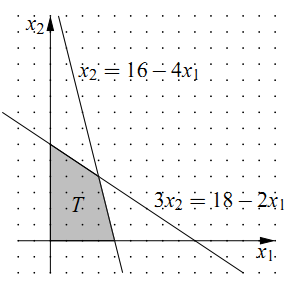
\includegraphics[height=6cm]{./kepek/2valtozo_megoldas_rajz.png}
\quad 
\subfigure{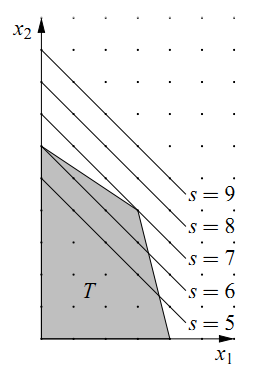
\includegraphics[height=6cm]{./kepek/2valtozo_megoldas_terulet.png} }}
\caption{Kétváltozós feladat grafikus megoldása} \label{fig:KetValtGraf}
\end{figure}

Ha a célfüggvényt különböző $x$--re felrajzoljuk meghatározható az optimális
megoldás és az ehhez tartozó $x$ értékek. Egy alternativ megkőzelités, hogy
vesszük célfügvény irányvektor normálját és ennek irányából pásztázunk végig a
meghatározott konvex sokszögben, a metszőpontok mentén. A megoldást az utolsó
megvizsgált metszőpont adja.

\subsection{Fourier-Motzkin elimináció}

Ennek segítségével megvizsgálhatjuk az egyenlet megoldhatóságát: $n$ változós
egyenletet visszavezetjük $n-1$ változóra, iteratívan, amíg egy változós
egyenletrendszert nem kapunk; erre könnyű megoldhatóságot vizsgálni. A folyamat:

\begin{enumerate}
  \item Minden egyenlet $\alpha \in \mathbb{R}^+$ szorzással az alábbi alakra
  hozható:
  \begin{displaymath}
  \begin{bmatrix}
  1  & A_+ \\
  -1 & A_- \\
  0  & A_0
  \end{bmatrix}
  \begin{bmatrix}
  x_1 & 
  x'
  \end{bmatrix}
  \leq
  \begin{bmatrix}
  b_+ \\
  b_- \\
  b_0
  \end{bmatrix}.
  \end{displaymath}
  \item 
  \begin{itemize}
  	\item Ha $A_-$ üres ($=\emptyset$): 
  	\begin{align*}
  	1 \cdot x_1 + A_+ x'     &\leq b_+ \\
  	1 \cdot x_1 + \alpha x' &\leq \beta \\
  	x_1 			  &\leq \beta - \alpha x' 
  	\end{align*} 
    Ekkor válasszuk úgy $x_1$--t, olyan kicsire hogy az összes sora e feltétel
    teljesüljön. Ezután $A_+$ teljes sorai elhagyható, továbbá elég $A_0$
    sorait vizsgálni, elhagyva a baloldalon található nulla oszlopot ($n-1$
    változós eset).
  	
  	\item Ha $A_+$ üres ($=\emptyset$): 
  	\begin{align*}
  	-1 \cdot x_1 + \alpha x'     &\leq \beta \\
  	x_1 			  &\geq \alpha x' - \beta 
  	\end{align*} 
  	Ekkor válasszuk úgy $x_1$--t, olyan nagyra hogy e feltétel teljesüljön.
  	Ezután $A_-$ elhagyható.
  	\item Ha $A_- \neq \emptyset$ és $A_+ \neq \emptyset$ akkor legyen 
  	$i \in A_-$ egy sora, $j \in A_+$ egy sora, és képezzük az összes sora az
  	alábbi ősszeget (ez exponenciális egyenlet szaporodást jelent, e miatt az algoritmus
  	futási ideje is exponenciális):
  	\[
  	\left( \alpha_i + \alpha_j \right) \cdot x' \leq b_i + b_j 
  	\]
  	Ezzel visszavezettük a kérdést $n-1$ változós estre.
  \end{itemize}
 \item Ha $n=1$ és 
 \begin{align*}
 \exists~b_0 < 0 &\Rightarrow \mbox{nem megoldható} \\
 \not \exists~A_+ \mbox{ vagy} \not \exists~A_- < 0 &\Rightarrow \mbox{megoldható} \\
 \mbox{másképp igaz, hogy } x_1 \leq \beta_+ \mbox{ és } y_1 \geq \beta_-
 &\Rightarrow \mbox{megoldható ha } \mbox{max}(-\beta_-) \leq min(\beta_+)
 \end{align*} 
  Ha $n \geq 1$ folytassuk a $2$--es lépéstől.
\end{enumerate} 

A Gauss eliminációval szemben itt csak pozítiv skalárral szorozhatjuk be a sort,
az egyenlőtlenség miatt.
\newpage
\section{Farkas-lemma (két alakban). A lineáris program célfüggvény korlátossága.}

A következő egyenletekből csak a jobb vagy csak a bal egyenletrendszereknek
létezik egy időben megoldása:

\begin{enumerate}
  \item alak: \begin{align*}
  \overbrace{Ax \leq b}^{A1}  && \overbrace{yA= 0}^{A2}\\
   			 && y\geq 0 \\
             && yb\leq 0
  \end{align*}
  \item alak:\begin{align*}
  \overbrace{Ax = b }^{B1}   && \overbrace{yA \geq 0}^{B2}\\
  x \geq 0 && yb \leq 0 
  \end{align*}
\end{enumerate}

Legyen az alábbi mérettel rendelkező mátrixok:
\[
\overbrace{\begin{bmatrix} 1 &  \cdots &  n \end{bmatrix}}^{\hbox{y}} 
\overbrace{\begin{bmatrix} 1 & \cdots & n \\ \vdots & \ddots & \vdots \\ m  & \cdots & 0 \end{bmatrix}}^{\hbox{A}}
\underbrace{\begin{bmatrix} 1 \\ \vdots \\  n \end{bmatrix}}_{\hbox{x}}
\overbrace{\begin{bmatrix} 1 \\ \vdots \\  m \end{bmatrix}}^{\hbox{b}}.
\]

\subsection{1--es alak}
Az első alak két egyenletrendszere nem megoldható egy időben mert:
\[ 0 = 0x = (yA) \cdot x = y(Ax) \leq yb.\] E utolsó egyenlőtlenség nem
egyértelmű, ellenőrizni kell, hogy:
\[ Ax \leq b \Rightarrow y(Ax) \leq (yb).\] Szerencsére ez igaz lesz a mátrix
szorzás disztributív tulajdonsága miatt. Majd tovább futatva a korábbi
gondolatunkat $yb<0$ amely ellentmond a kiinduló feltételeknek.

Definiáljuk a következő $C$ halmazt, amely egy sorvektorok halmaza:
\[ C= \left\{ z \in \mathbb{R}^{n+1}, z = y (A|b), y \geq 0 \right\}, \].
Célunk bizonyítani, hogy létezik $C$-ben $(0, \cdots, 0 , <0)$ alakú sorvektor,
ha az egyenletrendszer nem megoldható.

A halmaz zártságára az alábbi lemmák igazak ($z_1, z_2 \in C, \lambda>0$):

\begin{itemize}
  \item $z_1+z_2 \in C$, mert $\begin{rcases}
  z_1=y_1(A|b) \\
  z_2=y_2(A|b) \end{rcases} \Rightarrow z_1+z_2=(y_1+y_2)(A|b)$ ahol $y_1+y_2 \geq 0,$
  \item $\lambda z_1 \in C$, mert $
  z=y(A|b) \Rightarrow \lambda z = \lambda y (A|b)$ ahol igaz, hogy $\lambda y \geq 0$.
\end{itemize}

$(A|b)$ sorai $\in C$ mert $y(i)=1$--el felvételt nyernek $C$--be. Most hajtsuk végre a
Fourier-Motzkin eliminációt $(A|b)$--re, úgy, hogy a nullákat nem töröljük:

\begin{displaymath}
\underbrace{
\begin{array}{|cccc|c|}
\hline
 &  &  &  & \\
 &  & &  & \\
A &  & &  &b \\
 &  & & &\\
\hline
\end{array}}_{\mbox{sorai } \in~C}
\Rightarrow
\underbrace{
\begin{array}{|c|ccc|c|}
\hline
0 &  &  &  & \\
\hline
0 &  & &  & \\
0 &  & &  & \\
\hline
0 &  & & &\\
\hline
\end{array}}_{\mbox{sorai } \in~C}
\Rightarrow
\underbrace{
\begin{array}{|ccc|c|c|}
\hline
0 &  0 &0  & +1  & b_+\\
\hline
0 &  0& 0&  -1& b_-\\
\hline
0 &  0& 0& 0& b_0\\
\hline
\end{array}}_{\mbox{sorai } \in~C}
\end{displaymath}

A zártsági lemma miatt az elimináció során a mátrix sorai $C$ halmazon belül
maradnak. Továbbá ha a feladat eredetileg nem megoldható a végén sem lesz az, ez 
meg két féle képen történhet meg:

\begin{itemize}
  \item Létezik $0 \cdot x_n \leq gamma$ egyenlet, ahol $\gamma < 0$. Ennek alakja 
  $(0,0, \cdots, 0, <0),$ tehát a sor $\in C$.
  \item $\begin{rcases}
  +1 \cdot x_n \leq \alpha_i \\ 
  -1 \cdot x_n \leq \alpha_j \\
  \end{rcases} \Rightarrow  \mbox{ ellentmondáshoz meg akkor jutunk ha }
  \alpha_i < -\alpha_j.$
  
  Az $i$ sor alakja $(0, \cdots, 0, +1, \alpha_i)$, a $j$ sor meg $(0, \cdots,
  0, -1, \alpha_j)$. Ennek az összege meg $(0, \cdots, 0, 0, \alpha_i+\alpha_j)$
  ami szintén $\in C$, mivel $\alpha_i+\alpha_j<0$.
\end{itemize}

\subsection{2--es alak}

Az, hogy a két egyenletrendszer ($B1$ és $B2$) közül csak az egyik megoldható
egy időben indirekt bizonyítjuk. Legyen $x,y$ egy--egy megoldás:

\[ 0 \leq \underbrace{
		   \underbrace{(yA)}_{\mbox{sorvektor}}x = 
		  y\underbrace{(Ax)}_{\mbox{oszlopvektor}}}
		  _{\mbox{nem triviális lépés}}=yb<0\] ahol ellentmondáshoz jutunk.



Az hogy ha az egyik nem megoldható a másik igen visszavezetéssel bizonyítjuk az
$1$--es alakra. Ehhez először is kibontjuk a $B1$ alakot:
\begin{displaymath}
\underbrace{
\begin{array}{|c|c|c|}
\hline
y_1 & y_2  & y_3\\
\hline
\end{array}}_{y'}
\underbrace{
\begin{array}{|c|}
\hline
A \\
\hline
-A\\
\hline
-I \\
\hline
\end{array}}_{A'}
\leq
\underbrace{
\begin{array}{|c|}
\hline
b \\
\hline
-b\\
\hline
0 \\
\hline
\end{array}}_{b'}
\end{displaymath}

Azt állítjuk, hogy ha ez nem megoldható, akkor a $ yA \geq 0$, $yb \leq 0$ páros
igen.

\begin{align*}
\exists~y' &> 0 \\
y_1 A + y_2 (-A) + y_3(-I) &= 0 \\
y_1 \cdot b - y_2 \cdot b + y_3 \cdot 0 &<0
\end{align*}

Tehát:
\begin{align*}
(y_1 - y_2) \cdot A &= y_3 \\
(y_1 - y_2) \cdot B &< 0.
\end{align*}

Ekkor legyen $y=y_1-y_2$ és ezzel megkaptuk a $B2$ alakot, azaz igaz, hogy ez
megoldható.

\subsection{Korlátosság}

Az alábbi három kijelentés ekvivalens:

\begin{enumerate}
  \item $cx$ felülről korlátos az $Ax \leq b$ megoldás halmazon.
  \item $\not \exists$ megoldása az $ \begin{cases}
  Az \leq 0 \\
  cz > 0
  \end{cases} $ egyenletrendszernek.
  \item ~$\exists$ megoldása a~~$\begin{cases}
  yA=c \\
  y \geq 0
  \end{cases}$ egyenletrendszernek.
\end{enumerate}

A tétel bizonyítását \aref{fig:KorBizKor} ábra szerint fogjuk belátni.
 
\begin{figure}[htbp]
\caption{A korlátosság bizonyítási kőrre}
\label{fig:KorBizKor}
\centering \begin{tikzpicture}[scale=1.7]
  \tikzset{ p/.style={circle,white,fill=gray,inner sep=0pt,minimum size=0.3cm},
  }
  \node[p] (1) at (0, 0) {1};
  \node[p] (2) at (-1.5, -1) {2}; 
  \node[p] (3) at (+1.5 , -1) {3};
  
  % the connection between the dots
  \draw[-latex] (1) -- (2) node [midway, above=2pt] {($\star$)}; 
  \draw[-latex] (3) -- (1) node [midway, above=2pt] {($\cdot$)}; 
  \draw[-latex] (2) -- (3) node [midway, below] {Farkas lemma $A^T,c^T$--re};
  \draw[-latex] (3) -- (2);
\end{tikzpicture} 
\end{figure}

\newcommand*\circled[1]{\tikz[baseline=(char.base)]{
            \node[shape=circle,draw,inner sep=1pt] (char) {#1};}}
            
\begin{description}
  \item[($\star$) -- \circled{1} $\Rightarrow$ \circled{2}:]  Legyen $x_0$
  megoldása az $Ax \leq b$--nek és tegyük fel, hogy mégis létezik megoldása
  \circled{2}--nek. Ekkor legyen $\lambda > 0$, $x_0 + \lambda z$ is megoldása
  az $Ax \leq b$--nek, mert:
  \[ A(x_0+ \lambda z) = Ax_0 + \lambda (Az) \leq A x_0 + 0 \leq b \] Továbbá
  $c(x_0 + \lambda z ) = c x_0 + \lambda (cz)$, és mivel $cz>0$ a $\lambda$
  alkalmas megválasztásával ez tetszőleges nagyá tehető. Ez meg ellentmond
  \circled{1}--nek, tehát feltevésünk hamis volt.
  \item[($\cdot$) -- \circled{3} $\Rightarrow$ \circled{1}:]  Legyen egy $y$
  ami teljesíti \circled{3}--at és $x$ ami megoldása \circled{1}--nek. 
  \[ cx = (yA)x = y(Ax) \leq yb \]
  Ekkor $yb$ felső korlát az $Ax$ megoldás halmazán $cx-re$, tehát \circled{3}--ból
  következik \circled{1}.
\end{description}

\skiptooddpage 
\section[A lineáris programozás dualitás tétele]{A lineáris programozás dualitás
tétele (két alakban), a lineáris programozás alapfeladatának bonyolultsága}

\subsection{A lineáris programozás dualitás tétele (két alakban)}
A tétel kijelenti, hogy ha: 

$ \begin{rcases}
\mbox{LP: max}\left\{cx:Ax \leq b\right\} \\
\mbox{megoldható} \\
\mbox{felülről korlátos}
\end{rcases} \Rightarrow$ $\begin{cases}
\circled{1} \begin{cases}
\mbox{DP: min} \left\{ yb:yA = c, y \geq 0 \right\} \\
	\mbox{megoldható} \\ 
	\mbox{alulról korlátos}  
\end{cases} \\
\circled{2} \begin{cases}
\mbox{LP--nek } \exists \mbox{ maximuma} \\
\mbox{DP--nek } \exists \mbox{ minimuma} 
\end{cases}\\
\circled{3} \mbox{ maximum } = \mbox{ minimum}
\end{cases}$

Ezzel ekvivalens alakja az LP és a DP-nek a:
\begin{align*}
\mbox{LP: max} &\left\{ cx:Ax \leq b, x \geq 0 \right\} \\
\mbox{DP: min} &\left\{ yb:yA \geq c, y \geq 0 \right\}.
\end{align*}

Az \circled{1}--est bizonyítottuk az LP korlátosságánál, a \circled{2} és 
\circled{3}--hoz felhasználjuk a következő \emph{lemmát}:

\[
\begin{rcases}
Ax \leq b \mbox{ megoldható} \\
t \in \mathbb{R} \\
Ax \leq b \mbox{--nek } \not \exists~x \mbox{ megoldása, hogy } cx \geq t
\end{rcases} \Rightarrow
\parbox[t]{6cm}{
$\{yA=c, y \geq 0\}$--nak $\exists$ olyan megoldása amelyre  $yb < t$.}
\] A lemma \emph{bizonyításhoz}, átfogalmazzuk a bal oldalt mint egy Farkas
lemma alak:
$\begin{cases} Ax \leq b \\
-cx \leq -t \end{cases}$, és tudjuk, hogy a rendszer nem megoldható (nem
létezzik $x$ ami teljesiti). Alkalmazzuk rá a Farkas--lemmát, ennek második
alakja felírható, mint ($\lambda \geq 0, y
\geq 0$):
\begin{align*}
\begin{bmatrix} y & \lambda\end{bmatrix}
\begin{bmatrix} A \\ -c \end{bmatrix} = yA - \lambda c = 0 &\Rightarrow 
yA = \lambda c, \\
\begin{bmatrix} y & \lambda\end{bmatrix}
\begin{bmatrix} b \\ -t \end{bmatrix} =yb~ - \lambda t < 0 &\Rightarrow 
yb < \lambda t
\end{align*}

Ha $\lambda=0 \Rightarrow \begin{rcases}
yA = 0, \\
y \geq 0, \\
yb <  0 \end{rcases} \xRightarrow{\text{Farkas--lemma}}$ $Ax \leq b$ nem
megoldható, de ez ellentmondás az állításnak, tehát $\lambda$ nem lehet nulla
($\lambda \neq 0$). Legyen $y'=\frac{1}{\lambda}y$ így az egyenletrendszer
$y'A=c,~y'\geq0,~y'b<t$ alakú lesz és ezzel megadtunk minden $y$--ra egy
$y'$--et amely teljesíti a lemma kijelentését.

A \circled{2} \emph{bizonyításához} tegyük fel, hogy $\not \exists$ maximum
LP--n, ekkor legyen $t=\mbox{sup}\left\{cx:Ax \leq b \right\}$ (hiszen bármely
$x \subseteq R, x \neq \emptyset, x$ felülről korlátosnak $\exists$ szuprémuma,
legkisebb felső korlátja, ha még maximuma nincs is). Ha $t$ nem maximum
$\Rightarrow Ax \leq b$--nek $\not \exists~cx \geq t$--t teljesítő megoldása.
Ekkor:

\[ cx = (yA)\cdot x = y (Ax) \leq yb < t.\]

Így $yb$ egy $t$-nél kisebb felső korlát $cx$-re, de ez ellentmondás, tehát t
nem szuprémum és feltevésünk hamis volt, létezzik maximum LP--n. A DP--n történő
bizonyításhoz használjuk fel az LP bizonyítást, átírva a feladatott max--ra ($E$
-- egység mátrix):

\[ max \left\{ (-b)^T y^T :
\begin{cases}
(~~A^T)y^T    &\leq~~c^T \\
(-A^T) y^T &\leq -c^T \\
(-E~~)y^T    &\leq~~0 \\
\end{cases}  \right\} \]
 
A \circled{3} \emph{bizonyításához} már láttuk, hogy a \[ \mbox{max}\left\{
cx:Ax \leq b \right\} \leq
   \mbox{min}\left\{ yb:yA = c, y \geq 0 \right\}
\] fennáll. Legyen $t=\mbox{min}\{ yb:yA~=~c, y~\geq~0 \}$ és tegyük fel, hogy a
fenti egyenlőtlenségben nem egyenlőség áll.  Tehát ekkor az LP--nek
$\not\exists~cx \geq t$ kifejezést teljesítő megoldása, amiből következik,
hogy a duális feladatnak van olyan megoldása amire $yb<t$. De ez ellentmondás t
választásának, tehát feltevéssünk hamis volt.

\subsection{LP bonyolultság}

Az LP feladat megfogalmazható, mint eldöntési probléma: $\exists?$ az $Ax \leq
b$--t kielégítő x vektor amelyre $cx\geq t$? A probléma NP--beli. Tanú egy ilyen
$x$. Ugyanakkor coNP--beli is, a duális feladat megoldása tanú erre. $x, y$
mérete véges.

\begin{description}
  \item[1947 -- Dantzig -- Szimplex módszer] Hatékony gyakorlati feladatokon, de
  exponenciális komplexitású.
  \item[1979 --  Hacsijan -- ellipszoid módszer] Polinomiális komplexitás, de
  gyakorlatban lassú.
  \item[1984 --  Karmakar -- belső pontos módszer]  Polinomiális, hatékonyabb az
  ellipszoidnál, de ez is a gyakorlatban lassabb a szimplexnél.
\end{description}
\newpage
\section{Egészértékű programozás: a feladat bonyolultsága, korlátozás és szétválasztás (Branch and Bound)}

\subsection{Egészértékű programozás}
A feladat:
\begin{align*}
IP &: \mbox{max }{cx: Ax \leq b, x \mbox{ egész}} \\
DIP &: \mbox{min }{yb: yA=c, y \geq 0, y \mbox{ egész}}
\end{align*}
\[ \mbox{max(IP)} \leq \mbox{max(LP)}= \mbox{min(DLP)} \leq \mbox{min(DIP)} \]

A feladat bonyolultságának meghatározásához fogalmazzuk át eldöntési problémára:
$\exists?~Ax \leq b,~ x$ egész között olyan vektor, amelyre $cx \geq t?$ Az IP
feladat NP--teljes. NP--beli mert x tanú. A dualitás tétel nem alkalmazható
mivel max(IP)~$<$~min(DIP) fent állhat, tehát a probléma nem coNP--beli. \emph{NP
teljes}, visszavezethető a $3$--SAT problémára.

A bizonyításhoz megadjuk a visszavezetést: definiálunk egy eljárást, amely tetszőleges
logikai függvényhez megad egy olyan IP problémát, melyre akkor és csak akkor igenlő a
válasz, ha a függvény kielégíthető. A függvény alakja:

\[ f(x_1, x_2, \cdots, x_k) = \bigwedge_{i=1}^{d}{\left( x_{i_1}^{e_{i_1}} \vee 
x_{i_2}^{e_{i_2}} \vee x_{i_3}^{e_{i_3}}\right).} 
\]
Az IP probléma ismeretlenjei legyen $z_{i=\overline{1,k}}$ egyenlőtlenségek, ahol 
$0 \leq z_{i=\overline{1,k}} \leq 1$. Továbbá minden diszjunkcióra is felírunk egy
egyenlőtlenséget:


\begin{align*}
z_{i_1} &+ z_{i_2} &+      z_{i_3}  &\geq 1 & \mbox{ ha }~~x_{i_1} \vee~~x_{i_2}\vee~~x_{i_3}& \\
z_{i_1} &+ z_{i_2} &+ (1 - z_{i_3}) &\geq 1 & \mbox{ ha }~~x_{i_1} \vee~~x_{i_2} \vee \neg x_{i_3}& \\
z_{i_1} &+ (1-z_{i_2}) &+ (1 - z_{i_3})  &\geq 1 & \mbox{ ha }~~x_{i_1} \vee \neg x_{i_2} \vee\neg x_{i_3}&\\
(1-z_{i_1}) &+ (1-z_{i_2}) &+ (1 - z_{i_3})  &\geq 1 & \mbox{ ha } \neg x_{i_1} \vee \neg x_{i_2} \vee \neg x_{i_3}&
\end{align*}

Ha $f$ kielégíthető, akkor $z_i=1 \Leftrightarrow x_i=$ ,,igaz''. Ez lesz az
egyenletrendszer egészértékű megoldása. 

Megfordítva, ha az egyenlőtlenség--rendszert egész $z_i$ értékkel ki tudjuk
elégíteni akkor -- mivel minden egész vagy $0$, vagy $1$ -- az $x_i$=,,igaz''
$\Leftrightarrow z_i=1$ választással $f$--et kielégítő értéket adtunk a logikai
változónak.

Eközben a $\sum_{i=1}^{k}{z_i}$ összeg értétek valahol $0$ és $k$ között adódik,
tehát $c=(1,1,\cdots,1)$ választással tulajdonképpen a \emph{,,Van-e az
$(1a-1b$) és a $*(2a-2d$ feltételeket kielégítő (egész) vektorok között olyan,
melyre $cx \geq 0$?''} kérdést tesszük fel. Az így kapott IP feladatra a válasz
akkor és csak akkor igenlő, ha az f kielégíthető.

\subsection{A korlátozás és szétválasztás az IP feladatra}

Alakja $\mbox{max} \left\{cx:Ax \leq b, f \leq x \leq g| x,f,g \in \mathbb{Z}^n
\right\},$ ahol az $f$ és $k$ korlátok, amelyek biztosítják, hogy a feladat véges
lépésben megoldható. A metódus kulcs gondolata, hogy az IP feladat megoldásához először
megoldjuk mint LP, ha az eredmény egész megvagyunk, egyébként tovább bontjuk két kisebb
IP feladatra. Legyen $z^*=cx^*$, az egyenlőtlenség mindig $Ax \leq b$ marad.

Az algoritmus folyamata:

\begin{enumerate}
  \setcounter{enumi}{-1}
  \item $\overbrace{L=\left\{ \left(
  \overbrace{f}^{\text{alsó}},\overbrace{g}^{\text{felső}},\overbrace{\infty}^{w
  \text{ -- maximum értéke}} \right) \right\}}^{\text{IP részfeladatok}},
  \overbrace{z^*=-\infty}^{\text{eddigi legjobb célfüggvény érték}},
  \overbrace{x^*}^{\text{legjobb megoldás}}$
  \item Ha $L=\emptyset \Rightarrow$ \emph{vége} és a megoldás az aktuális $z^*$
  és $x^*$.
  
  Egyébként $L$--ből vegyük ki IP$_i$ feladatott.
  \item Ha $w_i \leq z^*$, IP$_i$--nek a megoldása nem lehet $z*$--nál jobb,
  folytassuk az első ponttól (ez a \emph{Bound} lépés).
  \item Oldjuk meg a relaxált IP$_i$ feladatott (LP$_i$--t).
  \\ Ha $\not \exists$ megoldás visszalépünk az első ponthoz.
  \\ Egyébként: $z_i$ -- maximum érték,  $x_i$ -- maximum hely.
  \item Ha $z_i \leq z^*$, IP$_i$ feladat és rész feladatai maximum értéke is
  legfeljebb $z^*$, lépjünk vissza az első ponthoz.
  \item Ha $z_i > z^* \mbox{ és } x_i \in \mathbb{Z}^{n}$ akkor $ z^* = z_i, x^* =
  x_i$ (adat frissítés) és visszalépünk az első ponthoz.
  \item Választunk egy közbenső értéket $(f_{i_j} \leq t \leq g_{i_j})$ és egy
  ezt meghatározó $x_j$ elágazás változót $x_i$--ből ($j$ egy pozíció $x$
  vektorban, $i$ az IP feladat sorszámát jelöli). Ezután $L$--ben elhelyezzünk
  két új feladatott:  $(t+1, g, z_i)$ és $(f, t, z_i)$. Lépjünk vissza az első
  ponthoz (\emph{Branch} lépés).
\end{enumerate} 

Az algoritmus véges sok lépésben leáll és megtalálja a feladat optimumát. A
véges sok lépést $f$ és $k$ vektor garantálja, hiszen a kezdetben kitűzött
feladatnak csak véges sok rész problémája lehet a felhasznált korlátok miatt. Az
optimális részt indirekt bizonyítjuk: legyen $z_0$ az optimum, de az eljárás
$z*<z_0$--t kapta.

Állítjuk, hogy $L$--ben mindig kellet, hogy legyen olyan IP$_i$ feladat amelynek
az optimum értéke $z_0$. Ez kezdetben fent áll, és az algoritmus egy ilyen IP
feladattal a $5.$--ik vagy $6.$--ik lépéshez jut el. Ha az ötödikbe jut akkor az
algoritmus mégis csak megtalálja a $z_0$ optimumot, ami ellentmondás.

Ha a hatodik lépés következik be, akkor a két keletkező IP feladat közül az
egyikre teljesül, hogy a vizsgált tartományában a $z_0$--hoz tartozó optimum
benne van, így $z_0$ optimumot mindenképp megtaláljuk. Tehát az eljárás során a
lista sosem ürült ki, de ekkor az algoritmus sose állhatott volna le, ami a
keresett ellentmondás.

\subsection{Gyakorlati tanácsok}
\begin{itemize}
  \item LIFO alapú új feladat választás $L$--ből, mert a megoldás várhatóan
  mélyen van a fába és ez tud legmélyebbre leggyorsabban lenyúlni.
  \item Elágazásnál a legkevésbé egész $x_j$--t válasszuk elágazási változónak
  (amelynek törtrésze $\frac{1}{2}$-höz legközelebb van), közbülső értéknek
  pedig ennek egész értékét.
\end{itemize}
\newpage
\section{Totálisan unimoduláris mátrixok és alkalmazásai}

Egy totálisan unimoduláris mátrixn minden négyzetes részmátrixának determinánsa
$0, 1$ vagy $-1$. Ehhez szükséges (de nem elégséges) feltétel, hogy a mátrix
elemei is csak $0, 1$ vagy $-1$ lehetnek.

\[
\begin{rcases}
A \text{ totálisan unimoduláris -- TU} \\
b \text{ egész vektor} \\
c \text{ tetszőleges} \in \mathbb{R}^n \\
\text{max} \left\{ cx:Ax \leq b \right\} \text{ LP feladat}\\
\text{ami megoldható és véges}
\end{rcases} \Rightarrow \parbox[t]{8cm}{ Az IP feladat is megoldható és
maximuma megegyezik az IP feladat maximumával.}
\]

\emph{Lemma:} a totálisan unimoduláris tulajdonság megmarad, ha:

\begin{description}
  \item[sor vagy oszlopot $\cdot (-1)$] $\Rightarrow$ ekkor a determináns
  előjele változik meg.
  \item[egységvektor sor vagy oszlopként való hozzáadása] $\Rightarrow$ ha a
  mátrixhoz egységvektort veszünk hozzá például oszlopként, és egy kiválasztott
  négyzetes részmátrixában ez az oszlop szerepel, akkor az új oszlop szerinti
  kifejtésből azonnal látszik, hogy a determináns megegyezik az eredeti mátrix
  egy négyzetes részmátrixának determinánsával vagy annak ellentettjével, így
  értéke $0, 1$ vagy $-1$.
  \item[sor vagy oszlop ismétlés] $\Rightarrow$ ha a kiválasztott részmátrixba
  az eredeti is szerepel a determináns nulla lesz, ha csak az egyik marad, akkor
  előáll az eredeti mátrixból képzett részmátrix, amely determinánsának értéke
  megmarad $0, 1$ vagy $-1$. 
  \item[transzponáljuk] $\Rightarrow$ megmarad a determináns definiciójának
  következményeként.
\end{description}

\emph{Tétel. Bármely irányitott gráf illekszkedés mátrixa~\footnote{$ 
B(G_{(V,E)})=
b_{i_{\in V}j_{\in E}}=
\begin{cases}
0  & \text{ha a } j \text{--edik él nem illleszkedik az } i \text{--edik ponthoz,} \\
+1  & \text{ha a } j \text{--edik élnek az } i \text{--edik pont kezdőpontja,} \\
-1  & \text{ha a } j \text{--edik élnek az } i \text{--edik pont a végpontja,} \\
+1  & \text{ha a } j \text{--edik él az } i \text{--edik ponthoz illeszkedő hurokél.} \\
\end{cases}$} totálisan unimoduláris.}.\\

Irányitott illeszkedési mátrixnál az oszlopban $1$ van amely pontból indul az
él, $-1$ ahove mutat; hurokél esetébben egyetlen $1$--es található. A
bizonyitást teljes indukcióval. Legyen $M \in \mathbb{M}_{k\times k}$ méretű
részmátrix. Ha $k=1$ az állitás nyilvánvaló. Ha $k \geq 2$ és létezzik egy darab
oszlop amelybe legfeljebb egy nem nulla elem van, akkor kifejtés aszerint és az
indukció adja a többit. Másképp minden oszlopábban egy darab $+1$ és egy darab
$-1$ van. Így $M$ sorainak összege nullvektor $\Rightarrow$ det$M=0$.\\

\emph{Tétel. Páros gráf~\footnote{Páros gráfnak nevezünk egy $G$ gráfot, ha
csúcsainak halmazát fel tudjuk úgy osztani egy $A$ és $B$ halmazra, hogy az
összes $G$-beli élre teljesül, hogy az egyik végpontja $A$-ban van, a másik
pedig $B$-ben.} illeszkedési mátrixa totálisan unimoduláris.}\\ 

Mutason minden él $A$--ból $B$--be. Irányított gráf illeszkedési mátrixe TU. Az
eredeti illeszkedési mátriszának megkapásához $B$ csúcsainak megfelelő sorokat
$-1$--el szorozzuk.

\subsection{Maximális összsulyú párositás IP feladatként}

Legyen $x$ indikátor, hogy az él benne van e párositásban, $w$ egy tetszőleges
él súlyfüggvény és $B$ az illeszkedési mátrix (amely páros gráf lévén totálisan
unimoduláris). A \emph{feladat}, megfogalmazható mint max$\left\{ wx:Bx <= (1,
\cdots, 1)^T, x \geq 0 \right\}$. Az $x \geq 0 $ feltételt bevisszük $B$
mátrixba kiegészitve azt egy $m \times m$--es egységmátrix ellentettjével, de ez
nem változtat TU tulajdonságon. 

Az egyenlőtlenség így azt fejezi ki, hogy egy csucsból legfeljebb egy kiinduló
élet választunk ki, ami adja a párositás feladatát. 

\[
\begin{rcases}
B'=\begin{bmatrix} B \\ -I \end{bmatrix} \text{ TU} \\
b \text{ egész}
\end{rcases} \Rightarrow x \text{ egész vektor ($0$ vagy $1$) értékű -- IP feladat}
\]

A max$\left\{ wx : Bx \leq (1,\cdots,1)^T, x \geq 0 \right\}$ duálisa
min$\{ y(1,\cdots,1)^T : yB \geq w,$ $y~\geq~0\}$. Az $y$ megoldás
minden $v$ csúcshoz $c(v)$ címkét rendel, ahogy Egerváry Jenő párositás
algoritmusa is:

\[ yB \geq w \Rightarrow c(a) + c(b) \geq w(e), \forall e=\{a,b\}\in E.\]

\subsection{Intervallumgráf}

A számegyenes véges sok intervallum alkossa egy gráf csúcshalmazát, és két csúcs
akkor legyen szomszédos, ha a megfelelő intervallumok metszők; az így
meghatározott gráf az intervallumgráf. Felthető, hogy a gráfot meghatározó
intervallumok $n$--re az $[1,n]$ egész végpontú, zárt részintervallumai.

Legyen az $I=\left\{I_1, I_2, \cdots, I_n\right\}$ intervallumrendszer.
Rendeljük ehhez $n \times m$--es $A(I)$ mátrixot: sorai feleljenek meg az
$1,2,\cdots,n$ egészeknek, oszlopai peddig az I intervallumainak. Az $i$--ik sor
és a $j$--ik oszlop kereszteződésben akkor álljon $1$--es, ha $i \in I_j$, és
minden más helyen álljon $0$. \\

\emph{Tétel. Az így definiált A(I) mátrix totálisan unimoduláris.} \\

A bizonyitáshoz kiválasztunk egy tetszőleges $k \times k$ részmátrixot, majd
teljes indukciót használunk az egyesek darabszáma szerint. Ha nulla darab
egyesből áll a mátrix az nyilván TU. Ha ven benne két oszlop amelyben az első
egyes azonos helyen áll, akkor a nagyobb egyes darabszámúból kivonjuk a kisedd
darabszámot. Ez az egyesek darabszámát csökkenti, de a detereminását nem
változtatja.

Ha nincs ilyen szolop, de van csupa null oszlop, akkor a determináns nulla. Ha
egyik sem teljesül, akkor pedig be tudjuk rendezni az oszlopkat úgy, hogy az
alsó háromszögmátrixot kapunk oszlop cserével. Ez a művelet a determinánst csak
előjelbe változtatja meg, így a determináns egy vagy minusz egy marad. \\

\emph{Tétel. Az intervallumgráfok tetszőleges k színre megszinezhetőek
egyenletesen.}\\ 

Az egyenletesen alatt azt értjük, hogy ha $i$--t tartalmazó intervallumok száma
$d_i$, akkor ezek közül minden felhasznált szín esetén az ilyen szinű
intervallumok száma $\lceil \frac{d_i}{k} \rceil$~\footnote{felső egészrész}
vagy $\lfloor \frac{d_i}{k} \rfloor$~\footnote{alsó egészrész}.

Elég bebizonyitani, hogy az intervallumok közül kiválasztható néhány úgy, hogy
az intervallum közül kiválasztható néhány úgy, hogy bármely $1 \leq i \leq n$
esetén az $i$--t tartalmazó intervallumgráfok között $\lceil \frac{d_i}{k}
\rceil$ vagy $\lfloor \frac{d_i}{k} \rfloor$ darab kiválasztott legyen. Ekkor a
kiválasztott intervallumokat megszínezzük egy szsínnel majd elhagyuk őket, a
megmaradt intervalumra meg ugyanaz $k-1$--el.

Legyen:
\[\begin{rcases}
A=A(I) \\
d = n \text{ dimenziós vektor } i \text{--ik komponense } d_i \\
\lceil \frac{d}{k} \rceil \text{ vektor } i \text{--ik komponense} \lceil \frac{d_i}{k} \rceil \\
\lfloor \frac{d}{k} \rfloor \text{ vektor } i \text{--ik komponense} \lfloor \frac{d_i}{k} \rfloor \\
\lfloor \frac{d}{k} \rfloor \leq Ax \leq \lceil \frac{d}{k} \rceil, 0 \leq x \leq (1,\cdots, 1)^T
\end{rcases} \parbox[t]{6cm}{Megoldás: $x=\left( \frac{1}{k}, \cdots, \frac{1}{k} \right)^T$ ahol $A$
TU $\Rightarrow \exists$ egészértékű megoldás.} 
\]

$x$--ben $0$ és $1$ közötti elemek vannak, és egy komponense oszlop öszegge
$\lceil \frac{d}{k} \rceil$ és $ \lfloor \frac{d}{k} \rfloor$ között van. Így
ezeknap az oszlopoknak megfelelő intervalumukat kiválasztva valóbban $\lceil
\frac{d_i}{k} \rceil$ vagy $ \lfloor \frac{d_i}{k} \rfloor$ illeszkedi $i$--re.
\newpage
\section{A lineáris és egészértékű programozás alkalmazása hálózati folyamproblémákra.}

\[
\begin{rcases} 
G(V,E) \mbox{ irányított gráf} \\
s,t \in V \mbox{ két kitűntet csúcs} \\
c : E \mapsto \mathbb{R}^+ \mbox{ nem negatív kapacitásfüggvény}\\
x : E \mapsto \mathbb{R}^+ \mbox{ tetszőleges függvény}\\
\rho_x(v) \mbox{ -- } v\mbox{--be belépő élek összege } x \mbox{ szerint} \\
\delta_x(v) \mbox{ -- } v\mbox{--ből kilépő élek összege } x \mbox{ szerint}
\end{rcases} \parbox[c]{6.2cm}{ 
\begin{itemize}
  \item $x$ függvény akkor \emph{folyam}, ha \\ $\forall~v~\in~V - \{s,t\}$--re: \\ $\rho_x(v)=\delta_x(v)$
  \item $x$ megengedett, ha $\forall e \in E$--re $x(e) \leq c(e)$
  \item A folyam értéke: \\ $\delta_x(s)-\rho_x(s)=\rho_x(t)-\delta_x(t)$
\end{itemize}
 }
\]

\emph{Tétel. Ford Fulkerson: A maximális folyam értéke megegyezik a minimális vágás értékével.}

A bizonyításhoz először figyeljük meg a kővetkező lemmát: ha $x \in E \mapsto
\mathbb{R}^+$ és $\forall v \in V - \{s,t\}$ esetén $ \delta_x(v) \leq \rho_x(v)$
és $\delta_x(s) \leq \rho_x(t)$ akkor $x$ egy folyam. 

Ez igaz mert, ha $\forall v \in V-\{s,t\}$ csúcshoz felveszünk egy új terminálba
mutató élet, amelyekhez hozzárendeljük az $x'(e)=\rho_x(v)-\delta_x(v) \geq 0$
egyenletlőtlenséget (a belépők többségbe vannak a kilépőkhöz képest). A többi élen
maradjon meg a korábbi értékek, $x(e)=x'(e)$. 

Az így konstruált $x$ folyamhoz tartozik $G'$ gráf.  Mivel ez is folyam igaz,
hogy $\delta_{x'}(t) = \rho_{x'}(t)$. Ugyanakkor $ \rho_{x'}(t) \geq \rho_x(t)$
és $\delta_{x'}=\delta_{x}s$. Mivel csak egyenlőség állhat, ezért
$\rho_{x'}(t)=\rho_{x}(t)$. Hogy ez igaz legyen $x$ folyam kell, hogy legyen.


\begin{wrapfigure}{L}{0.35\textwidth}
  \begin{center}
    \vspace{-1.3cm}
\begin{displaymath}
\underbrace{
\begin{array}{c|ccc|c|}
\cline{2-5}
   &   & & & \\
   &  B& & & \\
 s &   & & &-1 \\
 t &   & & & 1 \\ 
 \cline{2-5}
   &   & & & 0 \\
   & E & & & 0 \\
\cline{2-5}
\end{array}}_{B^*}
\underbrace{
\begin{array}{|c|}
\hline
x\\
\\
\hline
\mu\\
\hline
\end{array}}_{x^*}
\leq
\underbrace{
\begin{array}{|c|}
\hline
\\
0\\
\\
\hline
\\
c\\
\\
\hline
\end{array}}_{M}
\end{displaymath}
  \vspace{-1.3cm}
  \end{center}
\end{wrapfigure}

AZ LP felíráshoz először is egészítsük ki a gráfot egy $e^*=(t,s)$ pszeudó éllel, ez lesz 
később majd a folyamértéke, $\mu$. Az így kapott gráf illeszkedési mátrixa legyen $B^*$.
Minden $v \in V - \{s,t\}$ csúcshoz tartozik egy sor, amelyre teljesül a $b_vx\leq 0$ feltétel 
(azaz a belépő élek ősszege nem kisebb, mint a kilépőké, mert $\delta_x(v) - \rho_x(v) \leq 
0 \rightarrow \delta_x(v) \leq \rho_x(v)$). 

A $B^*x^* \leq 0$ rendszer alapján $\begin{rcases} \delta_x(s)-\mu \leq 0 \\
\mu - \rho_x(t) \leq 0 \end{rcases} \Rightarrow \delta_x(s) \leq \mu \leq
\rho_x(t)$. Az előző lemmából meg következik, hogy $\delta_x(s)=\mu=\rho_x(t)$, 
vagyis, hogy a folyam értéke $\mu$. 

A maximális folyam max$\{ (0, \cdots,0,1)x^* : B^*x^* \leq 0; x^* \geq 0;$ $x
\leq c \}$. Az utolsó feltételt is hozzávesszük a mátrixhoz, mint az $E$ egy
egységvektor és a hozzá tartozó $c$ rész a $M$ vektorban.

A feladat duálisa min$\{ y(0, 0, \cdots, 0, c) :yM \geq (0, 0, \cdots, 0, 1);$
$y \geq 0 \}$. Fejezzük ki $y$--t mint $\left( \pi\left(v\right) |
w\left(e\right)\right)$.
Ekkor: $\begin{cases} 
(1)~\pi(v) \geq 0 \mbox{ és } w(e) \geq 0, \\
(2)~\mbox{minden } e = (u,v) \mbox{ élre }  \pi(u)-w(e) \geq 0, \\
(3)~\pi(t)-\pi(s) \geq 1. \end{cases}$ 

A duális változói közül $\pi$ a csúcsokhoz (menyivel nőt a potenciál), $w$ az
élekhez rendelhető (menyibe kerül nekem a szállitás az él mentén). A duális
feladat célja a $m_{\text{DLP}}= \mbox{min} \left\{ \sum_{e\in E}^{}
w(e)c(e)\right\}$ alak minimalizálása. Állítjuk, hogy ez megegyezik a hálózati
folyam minimális vágásának értékével (legyen ez $m_{\text{C}}$).

Bármely adott $m_{\mbox{C}}$ vágáshoz könnyen készíthető olyan $\pi$ és $w$
amelyre az $m_{\text{C}}= \mbox{min} \left\{ \sum_{e\in E}^{} w(e)c(e)\right\}$
következik. Bizonyításként adunk egy módszert ehhez: legyen $S$ (tartalmazza a
forráspontot) és $T$ (tartalmazza a terminál csúcsot) diszjunkt halmazok, ekkor:
$\begin{cases}
v \in S &\Rightarrow \pi(v)=0, \\
v \in T &\Rightarrow \pi(v)=1, \\
e \in (S,T) \mbox{ él } &\Rightarrow w(e)=1, \\
\mbox{másképp} &\Rightarrow w(e)=0.
\end{cases}$

Erre teljesül a $m_{\text{C}}= \mbox{min} \left\{ \sum_{e\in E}^{}
w(e)c(e)\right\}$, amiből adódik az $m_{\mbox{DLP}} \leq m_{\mbox{C}}$, már csak
a másik irányú egyenlőtlenséget kell beállítani. Az $M$ mátrix totálisan
unimoduláris, tehát $y$ is egész értékű elemekből áll (mivel a duális
feladatban, min$\left\{ yb:yA=c; y\geq 0 \right\}$, szereplő $c$ is az).

Legyen adott $(\pi,w)$ optimális, egészértékű megoldás, ebből kiindulva
elkészítünk egy $(\pi',w')~0$ vagy $1$ értékű optimális megoldást. Definiáljuk a
következő függvényeket:
$\pi'(v)=
\begin{cases}
0, &\mbox{ha } \pi(v) \leq \pi(s), \\
1, &\mbox{egyébként}, 
\end{cases}$ és
$w'(e)=
\begin{cases}
0, &\mbox{ha } w(e)=0, \\
1, &\mbox{ha } w(e) \geq 1.
\end{cases}$ 

Ekkor $(\pi',w')$--re $(1)$ és $(3)$ teljesül. A $(2)$-öt indirekt bizonyítjuk.
Tegyük fel, hogy egy adott $e=(u,v)$ él esetén $\pi'(u)-\pi'(w)+w'(e)<0$, ekkor
a $0-1$ érétkűségük miatt $\pi'(u)=w'(e)=0$. Ez $\pi'(v)=1$ esetben valósulna
meg, amikor $\pi'$ definíniciója miatt $\pi(v) > \pi(s) \geq \pi(u)$, ami
ellentmondana $(2)$--nek, mert $w'$ definíciója miatt $w(e)=0$. A megoldás
optimális mert $\sum w'(e)c(e) \leq \sum w(e)c(e)$, mivel $w'(e) \leq w(e)$.

Most visszatérve az $S$ és $T$ halmazainkra legyen, $S=\{v \in V: \pi'(v)=0\} $
és $T=\{v \in V: \pi'(v)=1\}$. Egy adott $e=(u \in S, v \in T)$ élre $w'(e)=1$.
Minden más élen $w$ csak akkor lehet egy, ha $c(e)=0$, mert egyébként $w'(e)=0$
változtatása után a feltételek továbbra is fennállnának, de a $\sum w'(e)c(e)$
csökkenne. Ezért $S$ és $T$ között feszülő élek alkotta vágás értéke
$m_{\mbox{DLP}}$, így $m_{\mbox{c}} \leq m_{\mbox{DLP}}$.

Ezzel egy általános bizonyítást adtunk a Ford--Fulkerson tételre, amely így
átfogalmazott alakban általánosabb kérdések megválaszolására is alkalmazható.

\subsection{Minimális költségű folyam keresése}

Minden élhez rendeljünk egy k költséget, amely kifejezi, hogy egy egységnyi folyam
átviteli azon menyibe kerül. Ekkor kitűzhető egy olyan feladat, ami a legalább $M$
nagyságú folyamok között keres minimális költségűt. Lineáris programozás alakban:

\[ \mbox{min} \left\{kx: B^*x^* \leq 0, x^* \geq 0, x \leq c,mu \geq M \right\}. \]

Ha az élek kapacitásai egész értékűek, akkor egész értékű folyam is választható.
Ha az élek költsége is egészértékű, akkor ismert hatékony algoritmus megoldására,
Ford--Fulkersontól.

\subsection{Többtermékes folyam}

Adott egy $G=(V,E)$ irányított gráf és abban k darab pontpár:
$(s_i,t_i)_{i = \overline{1,k}}$. $G$--t továbbra is képzelhetjük út-- vagy
csőhálózatnak, az $(s_i, t_i)$ pontpárok pedig a $k$ darab szállítandó termék
termelő--, illetve fogyasztóhelyének felelnek meg. Végül legyen adott egy $c:E
\mapsto \mathbb{R}^+$ kapacitásfüggvény.

A feladat egy megoldása abból áll, hogy minden élhez $k$ darab számot fogunk
hozzárendelni, megmondva, hogy az egyes termékből ott éppen mennyi halad át.
Erre az esetre is alkalmazható a lineáris programozás, sőt a legalább két
termékes folyamoknál már az egyetlen ismert hatékony algoritmus ($k=1$--re a
javító utas algoritmus egész értékű megoldást ad polinomiális időben). Az egész
értékű feladat viszont már itt is NP nehéz (mivel a feladatott leíró mátrix nem
totálisan unimoduláris ekkor).

\chapter{Matroidok}
\section{Matroid definiciója és a rangfüggvény szubmodularitása}

A matroidot definiálhatjuk a függetlenségi axiómákkal mint, legyen $E$ egy
tetszőleges és véges alaphalmaz. Ugyanakkor $F \subseteq  2^E$ egy halmaz
rendszer. Egy adott $M=(E,F)$ struktúra matroid, ha teljesül, hogy:

\[
\begin{cases}
\mbox{F1}) &\emptyset \in F \\
\mbox{F2}) &\begin{rcases}
X \in F \\ 
Y \subseteq X 
\end{rcases} \Rightarrow \parbox[L]{11cm}{$Y \in F$
($F$ \emph{leszálló halmazrendszer} -- ha egy halmaz benne van $F$--ben akkor annak összes
részhalmaza is benne van $F$--ben, ehhez szükséges az F$1$ axióma).
} \\
\mbox{F3}) &\begin{rcases}
X,Y \in F\\
|X| > |Y| \\
\end{rcases} \Rightarrow\parbox[t]{10.5cm}{ $\exists~x \in X-Y$,~hogy $Y \cup \{x\}
\in F~($\emph{szubmodularitás, kölcsönösen bővithetőség} -- legyen két halmazrendszer
a matroidból, ahol ez egyik számoságban több elemet tartalmaz; ha e több
eleműben létezik olyan elem amely a kisebbikben nincs, akkor ezzel a kisebbiket
kiegésztive szintén $F$--beli elemet kapunk).}
\end{cases}
\]

Egy $M=(E,F)$ matroidban: 

\begin{description}
  \item[független halamaznak] nevezzük $E$ alaphalmaz $F$--hez tartozó
  részhalmazait ( tehát $X\subseteq E$--re $X \in F$).
  \item[maximális független halmaznak] nevezzük azt az $X \in F$ halmazt
  amelyhez már nem bővithető tovább anélkül, hogy a halmaz függetlensége
  sérüljön.
  \item[matroid bázisai] a matroid maximális független halmaza.
  \item[minimálisan összefüggő halmaznak] nevezzük azt az $X \ in F$ halmazt
  amely nem független, de amelyből bárhogy veszünk el egy elemet a művelet
  függetlené tesszi.
  \item[körnek] nevezzük a minimálisan összefüggő halmazt.
  \item[hurok] az egyelemű kör. 
  \item[a halmaz rangja] egy $X\subseteq E$ halmaznak az $X$ maximális
  független részhalmazának mérete, elemszáma. Jelölése: $r(X)$.
  \item[a matroid rangja] az alaphalmaz rangja, azaz $r(E)$, ahol $r:2^E \mapsto \mathbb{Z}^+$.
\end{description}

\emph{Legyen $M=(E,F)$ matroid ahol $A\subseteq E$ és $X_1,X_2 \in A$ maximális
független halmazok $A$--ban (bázisok), akkor $|X_1|=|X_2|$}. A bizonyitás
indirket megy, legyen $|X_1| > |X_2| \Rightarrow \exists e \in X_1-X_2$, ahol
F$3$ miatt $X_1\cup \{e\} \in F \Rightarrow X_1$ nem maximális. De ez
ellentmondás, tehát a feltevéssünk is hamis volt.

\begin{table}[htbp]
\begin{center}
\caption{Példák matroidra}
\begin{tabular}{>{\centering\arraybackslash}m{7cm}>{\centering\arraybackslash}m{4cm}>{\centering\arraybackslash}m{1.5cm}}
Lineáris (mátrix) matroid & Grafikus matroid & Uniform matroid \\ \hline
$
\left( \begin{array}{ccc}
\overbrace{1}^a & \overbrace{2}^b  \\
0 & 0
\end{array} \right)
$ &
\centering
\begin{tikzpicture}[scale=1]
  \tikzset{ p/.style={circle,white,fill=gray,inner sep=0pt,minimum size=0.3cm},
  }
  \node[p] (1) at (0, 0) {};
  \node[p] (2) at (0, -1) {}; 
  
  % the connection between the dots
  \draw[bend left,-]  (1) to node [midway, right] {$a$} (2); 
  \draw[bend right,-]  (1) to node [midway, left] {$b$} (2);
\end{tikzpicture}
& $U_{2,1}$ \\ \hline
$
\left( \begin{array}{ccc}
\overbrace{1}^a & \overbrace{0}^b & \overbrace{1}^c  \\
0 & 1 & 1
\end{array} \right)
$ &
\centering
\begin{tikzpicture}[scale=1]
  \tikzset{ p/.style={circle,white,fill=gray,inner sep=0pt,minimum size=0.3cm},
  }
  \node[p] (1) at (0, -3) {};
  \node[p] (2) at (-1, -1) {}; 
  \node[p] (3) at (+1 , -1) {};
  
  % the connection between the dots
  \draw[-] (1) -- (2) node [midway, above] {$c$}; 
  \draw[-] (2) -- (3) node [midway, below] {$b$}; 
  \draw[-] (3) -- (1) node [midway, above] {$a$};
\end{tikzpicture}
& $U_{3,2}$ \\ \hline
$ \left( \begin{array}{ccccc}
\overbrace{1}^a & \overbrace{0}^b & \overbrace{1}^c & \overbrace{2}^d& \overbrace{0}^e  \\
0 & 1 & 1 &0&0
\end{array}  \right)
$
&
\centering
\begin{tikzpicture}[scale=1]
  \tikzset{ p/.style={circle,white,fill=gray,inner sep=0pt,minimum size=0.3cm},
  }
  \node[p] (1) at (0, -3) {};
  \node[p] (2) at (-1, -1) {}; 
  \node[p] (3) at (+1 , -1) {};
  \node[p] (4) at (+1 , -1) {};
  \node[p] (5) at (+1 , -1) {};
  
  % the connection between the dots
  \draw[-] (1) -- (2) node [midway, above] {$c$}; 
  \draw[-] (2) -- (3) node [midway, below] {$b$}; 
  \draw[-] (3) -- (1) node [midway, above] {$a$};
  \draw[bend left,-]  (3) to node [auto] {$d$} (1);
   \path (2) edge[loop left] node[left] {e} (2);
\end{tikzpicture}
& $|E|=5,$ $32$ részhalmaz\\ \hline
$ \left( \begin{array}{ccccc}
\overbrace{1}^a & \overbrace{0}^b & \overbrace{1}^c & \overbrace{1}^d\\
0 & 1 & 1 &2
\end{array}  \right)
$
& $\not \exists$
& $U_{4,2}$\\

\end{tabular}
\end{center}
\end{table}
 \begin{description}
  \item[Grafikus matroid] egy $G$ gráf által leírt $M=(G$ élei, $G$ --beli erdők). A bázis fogalma
  megfelel a feszítő erdőnek. Jelőlése $M(G)$ és még körmatroidnak is nevezzük.
  \item[Lineáris matroid] egy mátrix által indukált matroid $M=(A$ oszlopai, $A$ lineárisan
  független oszlopai). Mátrixmatroid név alatt is ismeretes.
  \item[Uniform matroid] egy $M=($ tetszőleges véges halmaz, a halmaz lefeljebb
  $k$ elemű részhalmazai). Legyen $n=|E|$. Ekkor $U_{n,k}$--val jelöljük az
  uniform matroidot. $U_{n,n}$ a teljes/szabad matroid (grafikusan egy csillag
  alakzat), ha összes részhalmaza független. $U_{n,0}$ a triviális matroid,
  amelyben csak az üres halmaz független (grafikusan minden éle egy hurok).
\end{description}

\subsection{Rangfüggvény szubmodularitása}
Bármely $X, Y \subseteq E$--re igaz, ha $r:2^E \mapsto \mathbb{Z}^+$ egy matroid
rangfüggvénye, akkor:

\[
\begin{cases}
\mbox{R1)}& r(\emptyset) = 0 \\
\mbox{R2)}& r(X) \leq |X| \\
\mbox{R3)}& r(Y) \leq r(X), \mbox{ ha } Y \subseteq X \\
\mbox{R4)}& r(X)+ r(Y) \geq r(X \cup Y) + r (X \cap Y)
\end{cases}
\]

Azaz (fordítva), ha $r$ egy egészérrtékű függvény $E$ részhalmazain, amelyre
teljesül a fenti négy tulajdonság, akkor $r$ egy $M=(E,F)$ matroid rangfüggvénye,
ahol:
\[F=\left\{ H : r(H)=|H| \right\}. \]

Az első három tulajdonság bizonyitása rögtön adódik a rang definiciójából. Az
R$4$--re meg (ami a rangfüggvény szubmodularitása) legyen egy $X,Y \in E$. $A$
egy maximálisan független halmaz $X \cap Y$--ban ($A \subseteq X \cap Y),$ amely
számossága $\alpha$. 

Nyilván $A$ kiterjeszthető egy B halmazzá úgy, hogy az maximálisan független
legyen $X \cup Y$--ban. Ehhez $X$--ből $\beta$ új elemet rakunk hozzá, és
$Y$--ból $\gamma$ darabot:
\begin{align*}
r(X \cap Y) &= \alpha \\
r(X \cup Y) &= \alpha + \beta + \gamma
\end{align*}

E számok korlátot szabnak $X$ és $Y$ rangjára is mint: 
\begin{align*}
r(X) &\geq \alpha + \beta \\ 
r(Y) &\geq \alpha + \gamma \\
r(X) + r(Y) &\geq \underbrace{\alpha + \beta + \gamma}_{r(X \cup Y)} + \underbrace{\alpha}_{r(X \cap Y)} \\
r(X) + r(Y) &\geq r(X \cup Y) + r(X \cap Y) \\
\end{align*}

Példa arra, hogy az egyenlőség nem mindig áll fent:
\vspace{0.4cm}

\begin{tabular}{>{\centering\arraybackslash}m{3cm}>{\centering\arraybackslash}m{6cm}}
\begin{tikzpicture}[scale=1]
  \tikzset{ p/.style={circle,white,fill=gray,inner sep=0pt,minimum size=0.3cm},
  }
  \node[p] (1) at (0, -3) {};
  \node[p] (2) at (-1, -1) {}; 
  \node[p] (3) at (+1 , -1) {};
  
  % the connection between the dots
  \draw[-] (1) -- (2) node [midway, above] {$c$}; 
  \draw[-] (2) -- (3) node [midway, below] {$b$}; 
  \draw[-] (3) -- (1) node [midway, above] {$a$};
\end{tikzpicture} 
& $
\begin{cases}
X=(a,b), &r(X)=2 \\ 
Y=(a,c) &r(Y)=2  \\
X \cup Y, &r(X \cup Y)=2 \\
X \cap Y, &r(X \cap Y) = 1
\end{cases}
$ \\
\end{tabular}

\section{Mohó algoritmus matroidon és matroid megadása bázissal, duális matroidok}

\[
\begin{rcases}
M=(E,F) \mbox{ matroid}, \\ 
w : E \mapsto \mathbb{R}^+
\end{rcases}
\xRightarrow{?} \parbox[L]{9.8cm}{mekkora a maximális összsulyú független halmaz,
azaz max$\left\{\sum_{e \in X}w(e)\right\}$ ha $X \in F$, és mely ez az $X$?}
\]

\vspace{0.4cm}
\emph{A mohó algoritmus tetszőleges matroid és súlyfüggvényre optimális
megoldást ad a fenti kérdésre, a $\emptyset \in F$--ből kiindulva, maximális
sulyú elemeket csökenő sorrendbe véve (amik nem sértik a halmaz
függetlenségét).}
\vspace{0.4cm}

A bizonyitás indirekt történik, tegyük fel, hogy nem. Legyen ekkor $Y$ az
optimumot meghatározó halmaz, $X$ pedig amit a mohó algoritmus adott. Tudjuk,
hogy $X$ és $Y$ is maximálisan független, tehát az F$3$ alapján $|X|=|Y|=n$. A
két halmaz elemeit rendezzük csökkenő sorrendbe, és írjuk fel őket mint
$X=\{a_1, a_2, \cdots, a_n\}$ és $Y=\{b_1, b_2, \cdots, b_n\}$, ahol:

\begin{align*}
w(a_1) \geq w(a_2) \geq \cdots \geq w(a_n) \\
w(b_1) \geq w(b_2) \geq \cdots \geq w(b_n) \\
\end{align*}

A mohó algoritmus a legnagyobb sulyú elemmet vesszi, amely esetén a
függetlenségi tulajdonság nem sérül, tehát az első elem a legnagyobb elem lesz,
azaz $w(a_1) \geq w(b_1)$. Mivel a két halmaz különböző egymástol, ezért lesz
egy $i$ index amire ez a feltétel megfordul, azaz $ w(b_i)> w(a_i)$, egyébbként
a mohó is az optimumot kapta volna meg. Amely lépésben ez előfordul a két halmaz
felírható mint:

\[
\begin{rcases}
A=\{a_1, \cdots, a_{i-1}\}, \\
B=\{b_1, \cdots, b_{i}\}
\end{rcases} 
\xRightarrow{\mbox{F3}} \exists~b_j \in B, \mbox{ amelyre } A + b_j \in F  
\]

Az $A$ halmaz elemei csökkenő sorrendbe vannak rendezve, tehát $w(b_j) \geq
w(b_i)$, de ugyanakkor itt $w(b_i) > w(a_i)$. De ez ellentmondás, mert ekkor a
mohó algoritmus a $b_j$ elemet választotta volna, nem peddig az $a_i$--t, tehát
feltevéssünk hamis volt, a mohó algoritmus megadja az optimális megoldást.

\vspace{0.4cm}
\emph{Ha a mohó algoritmus optimális megoldást ad és F$1$,F$2$ függetlenségi axiómák
teljesülnek akkor F$3$ is igaz.}
\vspace{0.4cm}

A bizonyitás ismét indirekt, tegyük fel, hogy a mohó algoritmus optimális megoldást ad, de
F$3$ nem lesz igaz. Ilyenkor $X,Y \in F$, ahol $|X|>|Y|$ igaz, de $\not \exists~x \in X-Y$ úgy, hogy
$Y \cup \{x\} \in F$. Legyen:

\[
\begin{rcases}
r=\frac{|Y-X|}{|X-Y|}\\
w : E \mapsto \mathbb{R}^+ \\
w(e) = \begin{cases}
1 & e \in Y, \\
r + \frac{1-r}{2} & e \in X-Y, \\
0 & \mbox{másképp}
\end{cases}
\end{rcases}\Rightarrow
\parbox[L]{8.25cm}{
Az algoritmus elöszőr kiválasztja $Y$ elemeket, de ezután már csak nulla sulyút
választhatna. Így az összsúly ekkor $|Y|\cdot 1$. $X$ összsúly visszont $|X \cap
Y| + |X-Y|\cdot(r+\frac{1-r}{2})$, ami nagyobb. De így egy optimálisabb megoldást
kaptunk, azaz a mohó nem az optimumot adta meg. De ez elentmond a kiinduló feltételünknek,
tehát a feltvésünk, hogy $F$3 nem teljesül, hamis. } \]

\begin{figure}[htbp]
\centering
\begin{tikzpicture}
	\draw  (-1.5cm,1.5cm) node{X};
	\draw  (2.5cm,1.5cm) node{Y};
	\draw  (3.5cm,-1.5cm) node{$0$};
	\draw  (4.5cm,-2cm) rectangle (-2.5cm,2cm);
	\begin{scope}[opacity=0.8]
		\filldraw[fill=gray, draw=gray] (0,0) ellipse (2cm and 1.5cm) ;
		\filldraw[fill=lightgray, draw=lightgray] (2cm,0) ellipse (1.8cm and 1.2cm) ;
	\end{scope}
	\draw  (-1cm, 0) node[color=black]{$1-\epsilon$};
	\draw  (1cm, 0) node[color=black]{$1$};
	\draw  (2.5cm, 0) node[color=black]{$1$};
	\draw  (-1.0cm,0.8cm) node{$\gamma$};
	\draw  (1.2cm,0.8cm) node{$\alpha$};
	\draw  (2.4cm,0.8cm) node{$\beta$};
\end{tikzpicture}
\caption{Ha a mohó algoritmus megoldása optimális, akkor F3 teljesül}\label{fig:Mohó}
\end{figure}

\subsection{Bázisos megadás}
Legyen $B$ egy matroid bázisainak halmaza, ekkor teljesül, hogy:

\[
\begin{cases}
\mbox{B1)} & B \neq \emptyset \\
\mbox{B2)} & |X_1|=|X_2| \Leftarrow \forall X_1,X_2 \in B\\
\mbox{B3)} & \begin{rcases}
X_1, X_2 \in B \\
e_1 \in X_1
\end{rcases}\Rightarrow \exists~e_2 \in X_2, \mbox{hogy } X_1-e_1+e_2 \in B \\
\end{cases}
\]

Fordítva, ha $(E,B)$ egy halmazrendszer ahol a fenti három tulajdonság teljesül akkor $M=(E,F)$
matroidot alkot, ahol:

\[
F = \left\{H: H \subseteq C \mbox{ valamely } C \in B\mbox{--re}\right\}
\]

\subsection{Duális matroid}

\[
\begin{rcases}
M=(E,F) \mbox{ matroid}, \\
\mbox{bázisai } B=\{B_1, \cdots, B_n\}
\end{rcases} \Rightarrow
\parbox[L]{9cm} {
A duális matroid bázisai megfogalmazható mint $B^*=\{E-B_1, \cdots, E-B_n\}$.
Ez meghatározza $F^*$--ot, és duális matroidot mint $M^*=(E,F^*)$ jelöljük.}
\]

Bizonyitanunk kell, hogy az $M^*$ matroidra teljesülnek a függetlenségi axiómák.
F$1$ és F$2$ nyilvánvaló. F$3$--at kell belátni, azaz, hogy $X,Y \in F^*$ és
$|X|>|Y|$ esetébben létezzik $x \in X-Y$, hogy $Y+x \in F^*$. Legyen $B_X
\subseteq E-X$ és $B_Y\subseteq E-Y$ egy--egy $M$--beli bázis, amelyek a
definició alpaján léteznek.

Ha létezzik $X$--beli elem amely nincs benne $Y$--ban és $B_Y$--ban se, akkor
ezt hozzávéve $Y$--hoz ismét $F^*$--beli halmazt kapnánk. Ha ilyen nem létezzik akkor 
$X \subseteq B_Y \cup Y$ és

\[
|B_Y \cap X | = |X-(X \cap Y)| > |Y - (X \cap Y)| \geq |B_X \cap Y|.
\]

$B_X$ és $B_Y$ mérete megegyezik ($|B_X|=|B_Y|$), tehát $|B_Y-X| < |B_X-Y|$.
Most e két halmazra alkalmazzuk F$3$--at, azaz $\exists~z \in (B_X-Y)-(B_Y-X)$
eleme amelyre $(B_Y-X)+z$ független $M$--ben. Ezt a független halmazt egészitsük
ki bázisá, úgy, hogy $B_Y$--ból vesszünk hozzá új elemeket, jelöljük ezt
$B'$--el. $B'$ bázisába létezik elem $E-B_Y$--ból, tehát létezik olyan $B_Y$--beli elem 
amely nincs benne $B'$--ben. Legyen ez az elem $u$. E $u$ elemre $Y+u \subseteq E - B'$,
tehát $Y+u \in F^*$. Megkaptuk az elemet amire mindig igaz lesz F$3$, tehát a bizonyitás
teljes. 

\[(M^*)^* = M \]

\subsection{A duális matroid rangfüggvénye}

\[ r^*(X) = |X|-r(E)+r(E-X)\]

A bizonyitáshoz csupán le kell vezetni:

\begin{align*}
r^*(X) &= \mbox{max} \{ |X \cap Y| : Y \in F^*\}   = \mbox{max} \{ |X \cap Y| : Y \in B^*\}\\
       &= \mbox{max} \{ |X \cap (E-Z)| : Z \in B\} = |X| - \mbox{min} \{ |Z \cap X| : Z \in B\}\\
       &= |X| - (r(E)-\mbox{max}\{|W \cap (E-X)| : W \in B\}) \\
       &= |X| - r(E) + r(E-X)
\end{align*}

\newpage
\section{Elhagyás és összehúzás. Matroidok direkt összege, összefüggősége. T test felett
reprezentálható matroid duálisának T feletti reprezentálhatósága.}

Legyen $M=(E,F)$ matroidon $X \subseteq E$ halmazra definiáljuk a következő
műveleteket:
\begin{description}
  \item[elhagyás] az $M \setminus X=(E-X, F \setminus Y)$, ahol $F \backslash
  Y=\{Y\subseteq E-X, Y \in F\}$ (tehát az új matroidot úgy kapjuk, hogy
  alaphalmazból elhagyjuk az $X$--beli elemekt és a halmazrendszerből meg azon
  elemeket amelybe ezek részt vesznek).
  \item[összehuzás]  az $M / X=(E-X, F / X)$, ahol az $M/X$ rangfüggvénye felírható
  $r(Y)=r(X \cup Y) - r(X), Y \in  E-X$ alakban (ha kivesszük az alaphalmazból az
  összehuzott elemeket az új alaphalmaz -- $Y$ -- rangja egyenlő a teljes kezdeti alaphalmaz 
  -- $X \cup Y = E$-- és kivett alaphalmaz különbségével).
\end{description}

Az elagyások és az összehuzás műveletek prioritása azonos, tehát felcserélhető. $M$ matroid 
\emph{minora} annak egy elhagyás és összehuzás sorozata. Bármely matroid minora előáll
$N=(M \setminus A) / B$ alakban, ahol $A$ és $B$ diszjunkt halmazok.

\emph{Az elhagyás és az összehuzás duális művelet: $\begin{cases}
M^*/X=(M \setminus X)^*, \\
M^* \setminus X = (M / X)^*.
\end{cases}$}

A bizonyitáshoz elég az elsőt belátni, mert ha az igaz, mindkét oldal duálisát
véve és $M$ helyet $M^*$--ra alkalmazva azt következik a második kijelentés.
Tudjuk tehát, hogy az duális matroid összehuzásának ($M^*/X$) rangfüggvénye
(legyen ez $r_1$):

\begin{align*}
r_1(Y) &=\underbrace{r^*(X \cup Y)}_{|X \cup Y| + r(E-X-Y) - r(E)} - 
		 \underbrace{r^*(X)}_{|X| + r(E-X) - r(E)} \\
	   &= |Y| + r(E-X-Y) - r(E-X) 
\end{align*}

Ugyanakkor a matroidból X elhagyásával ($M^*/X$) a rangfüggvény ($r_2$):

\[ r_2(Y) = |Y| + r(T-Y) - r(T),\] ahol $T = E-X$ az $M\setminus X$ matroid
alaphalmazza. Látjuk, hogy $r_1(Y)=r_2(Y)\Rightarrow$ minden $Y$--ra a a két
matroid megegyezik, s ezzel bizonyitásunk teljes.

\begin{description}
  \item[direkt összeg] $\begin{rcases}
  M_1=(E_1,F_1) \mbox{ matroid}, \\
  M_2=(E_2,F_2) \mbox{ matroid}, \\
  E_1, E_2 \mbox{ diszjunkt, nem üres} \end{rcases} N = M_1+ M_2$ alaphalmaza
  $E_1 \cup E_2$, és $X \subseteq E_1 \cup E_2$ halmaz akkor független a direkt
  összegben, ha $X \cap E_1$ független $M_1$--ben és $X \cap E_2$ független
  $M_2$--ben. 
  \item[egy matroid \emph{összefüggő}] ha nem áll elő matroidok direkt
  összegeként. A grafikus matroid akkor összefüggő, ha a gráf kétszeresen
  összefüggő.
  \item[$M=(E,F)$ reprezentálható] T test felett, ha bármely elem az alaphalmazból
  $T$ feletti vektor. 
  \item[$M$ matroid koordinázható]T test felett, ha létezik olyan mátrix, amelynek oszlopai
  $T$ felett vektorok, és az ezek által meghatározott lináris matroid izomor $M$--el. 
\end{description}

Bármely $r=r(E), n=|E|$ matroidra létezzik $A \in \mathbb{M}_{r\times n}$ mátrix
amelyel leírható $M=(E,F)$ matroid (és a mátrix sorai lineárisan függetlenek).
Az $A$ mátrix megalkotásához $r$ sorra van szükség, ha a matroid több elemet
tartalmaz válaszunk ki $r$ lineárisan függetlent. Ekkor a jobb oldali alakra
hozható $A$ mátrix, ettől még ugyanazt a matroidot koordinázza:

\[
\overbrace{
\begin{array}{|lcr|}
\hline
1 & \cdots & r\\
\vdots  & \mbox{det} \neq 0 &\\
r &  & \\
\hline
\end{array}}^{\mbox{egység alaká alakít}}
\cdot~
\begin{array}{|lcr|}
\hline
1 & \cdots & n\\
\vdots  & A &\\
r &  & \\
\hline
\end{array}
=
\begin{array}{|lcr|}
\hline
1 & \cdots & n\\
\vdots  & B &\\
r &  & \\
\hline
\end{array}
=
\begin{array}{|lcr|lcr|}
\hline
1 & \cdots & r &1&\cdots&n-r\\
\vdots  & I_r &&\vdots&A'&\\
r &  & & r&&\\
\hline
\end{array}
\]

\emph{Ha $M=(E,F)$ matroid reprezentálható $T$ test felett akkor a duálisa ($M*$) is.}

A bizonyitáshoz hozzuk a matroid mátrixát oly alakra, hogy a mátrix bal oldalán
egy egységmátrix alakuljon ki. Legyen ennek $r$ sorra, ekkor $E_r$ egységmátrix
M egy bázisa, míg $A_0$ oszlopai a többi elemek. Megprobáljuk belátni, hogy $A'=(-A_0^T|E_{n-r})$
is reprezentálja a duális matroidot.

\colorlet{ColorGreyish}{black!10}
\[ 
M=
\begin{array}{|cc|c|c|rc|}
\hline
1       &  0     & \multicolumn{1}{>{\columncolor{lightgray}}l}{\color{black}0} & \multicolumn{1}{>{\columncolor{gray}}l}{\color{white}C} &     &\\
\vdots &  1     & \multicolumn{1}{>{\columncolor{lightgray}}l}{\color{black}0} &  \multicolumn{1}{>{\columncolor{gray}}l}{\color{white}} & A_0 &\\
0       &  \cdots  & \multicolumn{1}{>{\columncolor{ColorGreyish}}l}{\color{black}1} &\multicolumn{1}{>{\columncolor{lightgray}}l}{\color{black}}   &     &\\
\hline
\end{array}
\Rightarrow
M^*=
\begin{array}{|c|c|cc|lcr|}
\hline
\multicolumn{1}{>{\columncolor{gray}}l}{\color{white}}        & & 1&  &\multicolumn{1}{>{\columncolor{lightgray}}l}{\color{black}0} & \multicolumn{2}{>{\columncolor{lightgray}}l}{\color{black}}  \\
\multicolumn{1}{>{\columncolor{gray}}l}{\color{white}-C^T}    & &  & 1&\multicolumn{2}{>{\columncolor{lightgray}}l}{\color{black}} &\multicolumn{1}{>{\columncolor{lightgray}}l}{\color{black}0}  \\
\cline{1-1} \cline{5-7}
\multicolumn{1}{>{\columncolor{lightgray}}l}{\color{black}}   & &  &  & \multicolumn{1}{>{\columncolor{ColorGreyish}}l}{\color{black}1} & \multicolumn{1}{>{\columncolor{ColorGreyish}}l}{\color{black}} &\multicolumn{1}{>{\columncolor{ColorGreyish}}l}{\color{black}0}  \\
\multicolumn{1}{>{\columncolor{lightgray}}l}{\color{black}A_0^T}     & &  && \multicolumn{1}{>{\columncolor{ColorGreyish}}l}{\color{black}}  & \multicolumn{1}{>{\columncolor{ColorGreyish}}l}{\color{black}1}   & \multicolumn{1}{>{\columncolor{ColorGreyish}}l}{\color{black}} \\
\multicolumn{1}{>{\columncolor{lightgray}}l}{\color{black}} & &  &  & \multicolumn{1}{>{\columncolor{ColorGreyish}}l}{\color{black}0}  & \multicolumn{1}{>{\columncolor{ColorGreyish}}l}{\color{black}}  & \multicolumn{1}{>{\columncolor{ColorGreyish}}l}{\color{black}1} \\ \hline
\multicolumn{1}{c}{\mathsmaller{r-t}} & \multicolumn{1}{c}{\mathsmaller{t}} & \multicolumn{2}{c}{\mathsmaller{r-t}} & \multicolumn{3}{c}{\mathsmaller{n-2r+t}}
\end{array} 
\]

$M$ matroid és a duálisának a mátrixa természetes modón megfelelhetőek
egymásnak, az ábrán balról jobbra az oszlopcsoportok megfelelnek egymásnak.
Válaszunk ki az $M$ valamely bázisának megfelelő részmátrixot $A$--ban.
Feltehető, hogy ennek első $t$ oszlopa éppen $E_r$ utolsó $t$ oszlopa, míg a
maradék $r-t$ oszlop $A_0$ első $r-t$ oszlopa. Ennek a mátrixnak determinánsa
akkor nem nulla, ha $C$ determinánsa nem nulla. Mivel $B$ bázis, ezért $C$ nem
szinguláris.

$B^*=E-B$ elemeinek $A'$--ben az a mátrix felel meg, amely első $r-t$ oszlopa
$-A_0^T$, a többi pedig $E_{n-r}$ utolsó $n-2r+t$ oszlopa. Ennek a felső
blokk--háromszög mátrix determinánsa akkor nem nulla, ha $-C^T$ determinánsa nem
nulla.  Azaz, hogy $C$ nem szinguláris. Tehát a bázis komplementere is bázis, és
fordítva, és ezért $A'$ valóban a duálist reprezentálja.

\skiptooddpage 
\skiptooddpage 
\section{Matroid osztályok}

A következő matroid osztályokat különböztetjük meg: 

\begin{table}[htbp]
\begin{tabular}{|l|ll|}
\hline
Típus& Definició & Példa\\
\hline
\emph{grafikus} & ha egy $G$ gráf által indukált (körmatroid). & $K_3,K_5$ \\
\emph{kografikus} & a grafikus matroidok duálisa. & $K_3,K_5^*$\\
\emph{síkba rajzolható} & ha grafikus $\cap$ kografikus. &$K_3$\\
\emph{reguláris} & ha bármely test felett reprezentálható. & $K_{3,3}^*, K_5 \oplus K_5^*$\\
\emph{bináris} & ha csak a bináris test felett reprezentálható. & $F_7$\\
\emph{lineáris} & ha létezik test amely felett reprezentálható. & $F_7^-$\\
\emph{összes} & ha a korábbiak közül egyik se. & $F_7\oplus F_7^-$\\
\hline
\end{tabular}
\caption{Matroid osztályok}
\end{table}

Ugyanakkor igaz, az osztályokra, hogy grafikus, kografikus $\subseteq$ reguláris
$\subseteq$ bináris $\subseteq$ lineáris $\subseteq$ összes. 


\begin{wrapfigure}{l}{0.35\textwidth}
\caption{A Fano matroid}
\label{fig:Fano}
\centering \begin{tikzpicture}[scale=1]
  \tikzset{ p/.style={circle,white,fill=gray,inner sep=0pt,minimum size=0.3cm},
  }
  \draw [semithick,blue] (0,0) circle (1);
  \node[p] (1) at (0.85, 0.53)   {4};
  \node[p] (2) at (0, -1)        {6}; 
  \node[p] (3) at (-1.6 , -1)    {1};
  \node[p] (4) at (-0.85 , 0.53) {5};
  \node[p] (5) at (1.6 , -1)     {2};
  \node[p] (6) at (0 , 2)        {3};
  \node[p] (7) at (0 , 0)        {7};
  
  
  % the connection between the dots
  \draw[-] (1) -- (5); 
  \draw[-] (1) -- (6);
  \draw[-] (1) -- (7);
  
  \draw[-] (2) -- (3);
  \draw[-] (2) -- (5);
  \draw[-] (2) -- (7);
  
  \draw[-] (3) -- (4);
  \draw[-] (3) -- (7);
  
  \draw[-] (4) -- (6);
  \draw[-] (4) -- (7);
  
  \draw[-] (5) -- (7);
  
  \draw[-] (6) -- (7);
\end{tikzpicture} 
\end{wrapfigure}

A Fano matroid egy olyan matroid, amelyben az alaphalmaz mérete $7$ és minden
$2$ elemű részhalmaz független, de minden $3$ elemű csak akkor ha
\aref{fig:Fano} ábrán nincsenek egy körön vagy egy egyenesen. Ha kör megkőtést
elhagyjuk az így alkotott matroid az Anti--Fano matroid.

A Fano matroid pontosan azon testek felett reprezentálható amelyek
karakterisztikája $2$ (például a bináris matroid). Az Anti-Fano meg azon testek
felett amelyek karakterisztikája nem kettő. Tehát a két matroid direkt összege
semilyen test felett nem reprezentálható, azaz nem lineáris.

\vspace{0.4cm}
\emph{Grafikus matroid bármely test felett reprezentálható (reguláris).}
\vspace{0.4cm}

$\Rightarrow$ Induljunk ki egy $n$ pontú gráfból, tetszőleges irányitással,
rendeljünk minden ponthoz egy-egy $n$ dimmenziós egységvektort. Az élekhez
rendeljük a két végpontjuk közti különbséget (az irányitás lényegtelen). Azt
szeretnénk bebizonyitani, hogy egy élhalmaz akkor lineárisan független, ha az
általa kifeszített részgráf körmentes.

Az élek vektorjában csak $0,1$ vagy $-1$ áll, tehát ezzek bármely test felett
reprezentálhatóak. Ha a gráfban egy kör menti éleket összeadjuk null vektort
kapunk, mert a megfelelő nem nulla koordináták kiejtik egymást (az összeghez az
élet hozzáadjuk ha kör körbejárási iránya megegyezik az él irányával, és
kivonjuk egyébbként -- $1$ vagy $-1$ együthatók).

$\Leftarrow$ Fordítva, vegyünk egy összefüggő vektorhalmazt és ennek egy olyan X
nemüres részhalmazát amely olyan lineáris kombinációja ad nullát, ahol semelyik
együtható nem null. Az élvektorok azokon a koordinátákon nem nulla, amelyik
pontokat összeköt. 

Ahhoz, hogy a nullvektor kijöjjön miden ponthoz két darab nemnulla koordináta
kell, hogy létezzen. Azaz egy pontra két él illeszkedik, amely szerint minden
ilyen pont foka nagyobb mint $2$.  Egy adott részgráfban, ahol minden csúcs foka
nagyobb mint kettő, biztosan létezik kör.

\subsection{Tuttle tételei}

M matroid $\begin{cases}
\mbox{bináris} &\Leftrightarrow \mbox{ nem tartalmazza minorként: } U_{4,2}. \\ 
\mbox{reguláris} &\Leftrightarrow \mbox{ nem tartalmazza minorként: } U_{4,2}, F_7, F_7^*. \\
\mbox{grafikus} &\Leftrightarrow \mbox{ nem tartalmazza minorként: } \parbox[t]{4cm}{
$U_{4,2},$ $F_7$, $F_7^*$, $M^*(K_5)$, $M^*(K_{3,3})$.} \\
\end{cases}$

\subsection{Seymour tétel}

$M$ reguláris $\Leftrightarrow$  előáll $1$ grafikus, $1$ kografikus és egy
$R_{10}$ matroid példányából a direkt összeg, $2$-összeg és $3$-összeg műveletek
segítségével.

Az $R10$ egy $5$ rangú elem, egy $10$ elemű halmazon: nem grafikus és nem
kografikus.

\begin{figure}[htb]
\caption{Az $R_{10}$}
\label{fig:Seymour}
\centering \begin{tikzpicture}[scale=1]
\matrix [matrix of math nodes,left delimiter={(},right delimiter={)}]
{
1 & 1& 1& 1&  1 & 1 & 0 & 0 & 0 & 0\\
1 & 1& 1& 0 & 0 & 0 & 1 & 1 & 1 & 0\\
1 & 0& 0& 1 & 1 & 0 & 1 & 1 & 0 & 1\\
0 & 1& 0& 1 & 0 & 1 & 1 & 0 & 1 & 1\\
0 & 0& 1& 0 & 1 & 1 & 0 & 1 & 1 & 1\\
};\end{tikzpicture} 
\end{figure} 
\section{Matroidok összege, k-matroid-metszet probléma és bonyolultsága}

\[
\begin{rcases}
M_1=(E,F_1), \\
M_2=(E,F_2)
\end{rcases} 
\Rightarrow
M_1 \vee M_2  = (E,F'), X \in F' \Leftrightarrow X_1, X_2 
\begin{cases}
X=X_1 \cup X_2 \\
X_1 \in F_1\\
X_2 \in F_2
\end{cases}
\]

Tehát a matroid összegében azon elemek jelenek meg amelyek előállnak $F_1$ és
$F_2$--beli elemek uniójáként. 

\vspace{0.4cm}
\emph{Matroidok összege is matroid.}
\vspace{0.4cm}

A bizonyitáshoz ellenőrizzük a függetlenségi axiómákat. F$1$ és F$2$
nyilvánvaló, tehát csak F$3$--at látjuk be indirekt. Tegyük fel, hogy nem igaz, $X,Y \in F'$
és $|X|>|Y|$, de nem létezik $x \in X-Y$, hogy $Y+x \in F$. $X$ és $Y$
halmazokank mindig létezzik $X=X_1 \cup X_2~(X_1, X_2 \in F_1)$ és $Y=Y_1 \cup
Y_2~(Y_1, Y_2 \in F_2)$ felbontása.

\begin{figure}[htbp]
\centering
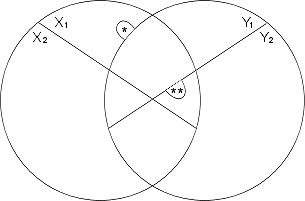
\includegraphics[width=0.4\linewidth]{./kepek/matroidosszeg.png}
\caption{Matroid összeg bizonyitás}\label{fig:Unif}
\end{figure}

Válasszunk egy olyan felbontást, hogy a részhalmazok diszjunktak legyenek,
$|X_1|>|Y_1|$ és az $|X_1 \cap Y_2|+|X_2+Y_1|$ összeg minimális értéket vegyen
fel. Ekkor $M_1$ matroidra alkalmazva az F$3$--at: létezik $x \in X_1-Y_1$,
hogy $Y_1+x \in F_1$.

Ha $x \not \in Y_2$ akkor $x+Y $ benne van az összegben $(\in F')$, ami
ellentmondana az indukciós feltevésünknek. Tehát $x \in Y_2$, amiből következik,
hogy létezik egy másik felbontás $Y=(Y_1+x) \cup (Y_2 -x)=Y_1^* \cup Y_2^*$.
Erre viszont a $|X_1\cap Y_2^*|+|X_2 \cap Y_1^*|$ összeg egyel kevesebb, ami
elentmond annak, hogy mi már a lehető legkisebbet választottuk korábban. Tehát a
feltvésünk hamis volt, F$3$ igaz.

\vspace{0.4cm}
\emph{$M=(E,F)$ matroid szabadmatroid, ha bármely részhalmaza független.}

\subsection{\texorpdfstring{Matroid metszet probléma -- MMP\textsubscript{$k$}}
			{Matroid metszet probléma -- MMPk}}

Adott $k$ darab matroid közös alaphalmazon: $M_i=(E,F_i)_{i=\overline{1,k}}$. A
kérédés amire keressük a választ, hogy létezik e $p \in \mathbb{N}$ konstansra
$p$ méretű halmaz $\cap F_i$--ben. Az eredmény nem minden esetben lesz matroid.

\vspace{0.4cm}
MMP$_2 \in $P.
\vspace{0.4cm}

A bizonyitáshoz induljunk ki egy adott $M_1=(E,F_1)$ és $M_2=(E,F_2)$ matroid
párból és legyen $p$ a halmazrendszerek metszetébben keresett halmazok mérete.
Ha $p>min(r_1, r_2)$ akkor a válasz nem, ilyen méretű halmaz nem létezik.
Másképpen csonkoljuk a két matroidot amig rangjuk min$(r_1,r_2, p)$--re nem
csökken:

\[ \begin{rcases}
M=(E,F) \mbox{ egy p rangú matroid} \\
0 \leq k \leq p \\ 
p \geq 1 
\end{rcases} \parbox[t]{5.5cm}
{$F' = \left\{ X \subseteq E: X \in F, |X| \leq k \right\}$ 
$(E,F')~M$ csonkolat matroidja} \]

Ezzel a problémát redukáltuk a közös bázis megkeresésére. $r_1=r_2=p$--re a
válasz akkor és csak akkor igenlő ha létezik ilyen méretű közös bázis, azaz ha
$M_1 \vee M_2^*=(E,2^E)$ szabad matroid.

$\Rightarrow$ Ha $M_1$ és $M_2$--nek van egy közös $B$ bázisa, akkor $M^*$--ban
$E-B$ bázis. Az $E=B \cup (E-B)$ egy felbontása az összegnek, azaz az összegben
$E$ független, tehát $M_1 \vee M_2^*$ szabadmatroid.

$\Leftarrow$ Legyen $E=C \cup D$ egy olyan felbontása a szabadmatroidnak, hogy
$C \in F_1$ és $D \in F_2^*$. Ekkor:
\[|E| \leq |C| + |D| = r_1(C) + r_2^*(D) \leq r_1(E)+r_2^*(E) = r_1(E) + |E| - r_2(E)=|E|. \]

Mivel $C$ és $D$--t diszjunkt halmazoknak választottuk, $C$ közös bázisa az $M_1$ és
$M_2$ matroidnak.

\subsection{Bonyolultság}

MMP\textsubscript{$k$} bonyolultsága ha $k \geq 3$--ra NP teljes. A feladat
NP--beli mert a $p$ elembeli halmaz közös tanú a két halmazrendszerre.

Az NP teljességhez figyeljük meg, hogy MMP\textsubscript{$3$} visszavezethető
Hamilton út keresésére (amiről tudjuk, hogy egy NP teljes probléma). Legyen $G$
irányított gráfban $u$ és $v$ között Hamilton út keresés:

\[
\begin{cases}
\begin{rcases}
M_1=(E,F_1) \\
X \subseteq E \\
X \in F_1
\end{rcases} &\Leftrightarrow \parbox[t]{10cm} {$X$ részgráfban minden pont
befoka legfejlebb egy, és az $u$ befoka nulla.} \\
\begin{rcases}
M_2=(E,F_2) \\
X \subseteq E \\
X \in F_2
\end{rcases} &\Leftrightarrow \parbox[t]{10cm} {$X$ részgráfban minden pont
kifoka kisebb vagy egyenlő eggyel egy és a $v$ kifoka nulla.} 
\end{cases}
\]

Ekkor M$_3$  a gráf körmatroidja, és M$_1$, M$_2$, M$_3$ közös $|V|-1$ elemű
bázisai $G$ gráf irányított Hamilton útjai.

\vspace{0.4cm}
\emph{MMP$_k$, ha $k>3$ NP teljes.} 
A bizonyitáshoz az imént konstruált struktúrához vegyünk hozzá $k-3$ darab
szabad matroidot.
\section{\texorpdfstring{A k-matroid partíciós probléma -- MPP\textsubscript{$k$}}
		 {A k-matroid partíciós probléma}}
			 
Adott $k$ darab $M_i = (E, F_i),$ ahol $i={\overline{1,k}}$ matroid. A kérdés,
hogy a matroidok összege ($\vee_{i=1}^{k}M_i$) a szabad matroidot ($E,2^E$) adja
e? Másképp megfogalmazva előáll e az alaphalmaz $E$ az $\cup_{i=1}^{k} E_i$ alakban,
ha $\forall i$-re $E_i \in F_i$. Feltehető, hogy az $E_i$ halmazok diszjunktak, így 
egy partíciós problémához jutottunk.

\vspace{0.4cm}
\emph{MPP$_k$ P-beli probléma.}
\vspace{0.4cm}

MPP$_k \in$ NP, mert ha a feladatnak van megoldása, az egy tanú, amely lineáris időben
ellenőrizhető. MPP$_k \in$ coNP, mert ha a feladatnak nem létezik megoldása, akkor
adhatunk rá egy $X \subseteq E$ halmazt, ami biztosan összefüggő az összegben, azaz 
$\sum r_i (X) < |X|$.

\subsection{Algoritmikus megoldás}

Most adunk erre egy algoritmust amely megoldja a feladatott, ehhez kiindul üres
halmazokból és addig bővíti azokat amíg uniójuk $E$ nem lesz. Ha egy adott
pontnál nem bővíthető tovább egyik halmaz sem, akkor az lesz a  keresett ellen
példa, ami bizonyítás arra, hogy a matroidok nem particionálhatók.

\begin{figure}[htbp]
\caption{Példa, hogy a mohó algoritmus miért nem működik: 
		  $E_1 = \{2\}$, $E_2 = \{3\}$ állapotban nem tudunk újabb élt 
		  belevenni egyik halmazba sem. Egy jó particionálás pedig a 
		  $E_1 = \{ 1 \}$, $E_2 = \{ 2, 3 \}$ felosztás.}
\label{fig:MPPMohoNem}
\centering \begin{tikzpicture}[scale=0.8]
  \tikzset{ p/.style={circle,white,fill=gray,inner sep=0pt,minimum size=0.3cm},
  }
  \node[circle, fill=white] (M1) at (-3,0.5)   {$M_1$};
  \node[p] (1) at (-2,0)   {};
  \node[p] (2) at (0, 0)     {}; 
  \node[p] (3) at (+2,0)   {};
  
  \node[circle, fill=white] (M2) at (9,0.5)   {$M_2$};
  \node[p] (4) at (4,0)   {};
  \node[p] (5) at (6, 0)     {}; 
  \node[p] (6) at (8,0)   {};
  
  % the connection between the dots
  \draw[bend left,-]  (1) to node [midway, above] {$2$} (2); 
  \draw[bend left,-]  (2) to node [midway, below] {$1$} (1);
  \draw[-]  (2) to node [midway, below] {$3	$} (3);
  
  \draw[bend left,-]  (4) to node [midway, above] {$3$} (5); 
  \draw[bend left,-]  (5) to node [midway, below] {$1$} (4);
  \draw[-]  (5) to node [midway, below] {$2$} (6);
\end{tikzpicture} 
\end{figure}

Az algoritmus egy $n+k$ pontú segédgráffal dolgozik ($|E|=n$ csúcs a halmazoknak
és $k$ csúcs a partícióknak), tehát $V' = E \cup \{p_1, p_2, \ldots, p_k\}$. A
gráf éleit definiáljuk mint $(\overrightarrow{xy}) \in E'$ ahol:

\begin{figure}[htbp]
\caption{Segéd gráf két halmazra}
\label{fig:MPP_graf}
\centering \begin{tikzpicture}[scale=1]
  \tikzset{ p/.style={circle,white,fill=gray,inner sep=0pt,minimum size=0.6cm},
  }
  \draw[lightgray] (0,0) rectangle(1.5,1.5);
  \draw[lightgray] (0,0) rectangle(-1.5,1.5);
  \node[circle,gray, fill=white] (E1) at (-1,0.2)   {$E_1$};
  \node[circle,gray, fill=white] (E2) at (+1,0.2)   {$E_2$};
  \path[fill=lightgray] (-1.5,0) arc [start angle=180, delta angle=180, radius=1.5];
  
  \node[p] (1) at (0,-1)   {$1$};
  \node[p] (2) at (-1,1)   {$2$};
  \node[p] (3) at (+1,1)   {$3$};
  \node[p] (p1) at (-1,2.5)   {$p_1$};
  \node[p] (p2) at (+1,2.5)   {$p_2$};
     
  \draw[-latex]  (1) -- (2);
  \draw[-latex]  (1) -- (3);
  \draw[-latex]  (2) -- (p2);
  \draw[-latex]  (3) -- (p1);
  
\end{tikzpicture} 
\end{figure}


\begin{itemize}
  \item  $\begin{rcases}
  x \in E \\
  y = \{ p_i \}  \\
  x \not \in E_i\\
  E_i \cup  \{x\}  \in  F_i \end{rcases}
  \parbox[t]{11cm}{Egy ilyen él azt jelenti, hogy $x$-et hozzávehetjük $E_i$-hez
   a függetlenség megsérétése nélkül ($\overrightarrow{xp_i}$ -- az ábra felsõ
  részen a $p_i$-kbe mutató élek).}$
  \item $\begin{rcases}
  x,y \in E \\
  x \not\in E_i, y \in E_i\\
   E_i \cup \{x\} \not\in F_i,\\ 
   E_i \cup \{x\} - \{y\} \in F_i
  \end{rcases} \parbox[t]{10cm}{Egy ilyen él azt jelenti, hogy $x$-et
  hozzávehetjük $E_i$-hez, ha $y$-t elhagyjuk belöle ($\overrightarrow{xy}$ --
  az ábra alsó részén lévõ élek).}$
\end{itemize}

\begin{enumerate}
    \setcounter{enumi}{-1}
    \item $\forall~i~E_i = \emptyset$ kezdeti állapot ($i=\overline{1,n}$). Erre
    igaz, hogy $E_i \in F_i$.
    \item Keressük meg a legrövidebb irányított utat $E-\cup_{i}E_i$--ből
    $\left\{ p_1, \cdots, p_k \right\}$--ba.
    
    \item Ha létezik irányított út akkor ez meghatároz egy módosítás-sorozatot,
    hogy melyik $E_i$-t hogyan kell módosítanunk. Az út utolsó éle egy $p_j$-be
    megy, a többi $E$-beli elemek között, vagyis összesen 1-gyel növeljük
    $E_i$-k elem számát.  Ha egy {\it legrövidebb} ilyen út mentén javítunk,
    akkor bizonyítható, hogy $E_i$-k a módosítások után függetlenek maradnak (mi
    nem bizonyítjuk).
    \item Különben megállunk, nemleges a válasz, és a tanú $X$ az $E- \cup Ei$--ből
    irányított úton elérhető pontok halmaza.
\end{enumerate} 

\begin{figure}[H]
\caption{Általános alakban}
\label{fig:MPP_halm}
\centering 
\begin{tikzpicture}[scale=0.8]
	\tikzstyle{vertex}=[draw,circle,fill=white,minimum size=3pt, inner sep=0pt]
 	\begin{scope}
		\draw (0,0) -- ++(6cm,0)
					-- ++(0,-3cm)
					-- ++(-6cm,0)
					-- (0,0);
		\foreach \x in {1,2,3} {
		\draw (\x*1.5,0) -- (\x*1.5,-3);
		}
		\draw (0.75,-1.0) node{$E_1$};
		\draw (2.25,-1.0) node{$E_2$};
		\draw (3.75,-1.0) node{$\dots$};
		\draw (5.25,-1.0) node{$E_k$};
		\draw (0,-3) .. controls (0,-5) and (6,-5) .. (6,-3);
		
		\draw (0.75, 0.5)  circle (0.5mm) node[above](1){$p_1$};
		\draw (2.25, 0.5)  circle (0.5mm) node[above](2){$p_2$};
		\draw (3.75, 0.5) node[above]{$\dots$};
		\draw (5.25, 0.5)  circle (0.5mm) node[above]{$p_k$};

		\draw (0.75, -2.0)  circle (0.5mm) node[left]{};
		\draw (2.25, -2.0)  circle (0.5mm) node[left]{};
		\draw (3.75, -2.0)  circle (0.5mm) node[left]{};
		\draw (5.25, -2.0)  circle (0.5mm) node[left]{};

		\draw (2.25, -4.0)  circle (0.5mm) node[left]{$x$};
		\draw[color=gray, dashed] (-1,0.15) rectangle (6.5,-5);
		\draw [color=gray] (-0.5,-2.4) node{$E$};
		\begin{scope}[opacity=0.8,>=latex]
			\draw (2.25, -4.0) [->, shorten >=2pt, shorten <=1pt, line width=1pt, color=gray] -- (0.75,0.5);
			\draw (2.25, -4.0) [->, shorten >=2pt, shorten <=1pt, line width=1pt, color=gray] -- (5.25,0.5);
			\draw (0.75, -2.0) [->, shorten >=2pt, shorten <=1pt, line width=1pt, color=gray, loosely dotted] .. controls (0.25,-	1) .. (0.75,0.5);
			\draw (0.75, -2.0) [->, shorten >=2pt, shorten <=1pt, line width=1pt, color=gray] -- (2.25,0.5);

			\draw (0.75, -2.0) [->, shorten >=2pt, shorten <=1pt, line width=1pt, color=black] -- (2.25,-2);
			\draw (2.25, -4.0) [->, shorten >=2pt, shorten <=1pt, line width=1pt, color=black] -- (0.75,-2);
			\draw (2.25, -4.0) [->, shorten >=2pt, shorten <=1pt, line width=1pt, color=black, loosely dotted] .. controls (4.7,-2) .. (5.25,0.5);
		
		\end{scope}
	\end{scope}
\end{tikzpicture}\end{figure}


\subsection{2-matroid-metszet probléma}

Adott $k$ matroid ($M_i=(E,F_i)$, ahol $i=\overline{1,k}$) és egy p egész szám.
A kérdés, hogy létezik e $F_i$--nek legalább $p$ méretű közös eleme?

Az így megfogalmazott probléma $k=2$--re MMP$_2$ komplexitása P--beli.
MPP$_k$--ra már beláttuk, hogy $P$--beli, MMP$_2$-őt meg megfogalmazhatjuk mint a
$M_1 \vee M_2^*$ összeg szabad matroid e?

\skiptooddpage 
\section{\texorpdfstring{$k$--polimatroid}
		 {k--polimatroid}}

Egy  $f:2^E \mapsto \mathbb{N}$ egy $k$--polimatroid rangfüggvénye, ha teljesül:

\[
\begin{cases}
\mbox{KP1})& r(\emptyset)=0\\
\mbox{KP2})& r(\{X\}) \leq k, \mbox{ ekvivalens alak } r(X) \leq k |X|  \\
\mbox{KP3})& X \subseteq Y \Rightarrow r(X) \leq r(Y)\\
\mbox{KP4})& r(X \cup Y) + r (X \cap Y) \leq r(X) + r(Y) \Leftrightarrow r(X \cup Y) \leq r(X) + k|Y| \\
\end{cases}
\]

Ha $r(\{X\}) \leq 1$, tehát $k=1$ akkor $r$ egy matroid rangfüggvénye. 

\subsection{\texorpdfstring{$k$--polimatroid matching probléma}
		 {k--polimatroid matching probléma}}


Ha $r$ egy $k$--polimatroid rangfüggvény és $X\subseteq E$--re $r(X)=k|X|$,
akkor $X$--et egy $k$--matching halmaznak nevezzük. A $k$--polimatroid matching
probléma felírható mint:

\[
\begin{rcases}
E \mbox{ alap halmaz} \\
r \mbox{ egy } k \mbox{--polimatroid rangfüggvény} \\
p \in \mathbb{N} \\
\end{rcases}  \xRightarrow {?\exists X \subseteq E}
\begin{cases}
r(X)=k|X| \mbox{, tehát X } k \mbox{--matching} \\
|X| \geq p 
\end{cases}
\]

Figyeljük meg pár speciális esetét a problémának:

\begin{itemize}
  \item Adott egy $G$ gráf és egy $t \in \mathbb{N}$. $\nu(G) \geq t$? \footnote{
   $\nu(G)$ a $G$ gráfban található független élek maximális száma.
  } A probléma $2$--polimatroid matchingként: $r(X)=|X$
  által lefedett pontok halmaza$| \leq 2|X|$.
  \item $\begin{rcases}
  \mbox{két matroid} \\
  t \in \mathbb{N}
  \end{rcases}$ létezik  e $X \subseteq E$: $\begin{cases}
  |X| \geq t \\
  X \in F_1 \cap F_2~(\mbox{matroid metszet probléma})
  \end{cases}$ 
  $2$--polimatroid matchingént megfogalmazva: $r(X)=r_1(X)+r_2(X) \leq 2|X|$
  \item A két korábbi problémát összevonva $\nu(G)$ egy adott $G$ páros gráfban?
  
  Hogy megfogalmazzuk $k$--polimatroid problémának felhasználjuk a fenti két
  feladatott. A páros gráf két csúcs halmaza legyen $A$ és $B$. $M_1$ grafikus
  matroidban két él párhuzamos ha létezzük közös pontjuk $A$ ponthalmazban.
  $M_2$ hasonlóan van definiálva $B$--re. 
\end{itemize}

\subsection{Bonyolultság}
Teljes általánosságban a probléma nem oldható meg polinom időben. Az általánosság
a függvény megadási módjára vonatkozik. $\forall x \subseteq E$--re egységnyi
idő alatt $r(X)$ értéke megtudható, de ettől eltekintve a $2$ polimatroid
rangfüggvényéről semmit sem tudunk.

Ennek bizonyításához induljunk ki egy $|E|=2n$ alaphalmazból és ennek egy
$|E_0|=n$ részhalmaza. Továbbá legyen az alábbi két polimatroid rangfüggvény:

\[
\begin{cases}
\forall X \subseteq E \mbox{ és } |X|<n, & r_1(X)=r_2(X)=2|X| \\
\forall X \subseteq E \mbox{ és } |X|>n, & r_1(X)=r_2(X)=2n \\
\forall X \subseteq E \mbox{ és } |X|=n \mbox{ és } X = E_0, & r_1(X)=r_2(X)=2n-1\\
\forall X \subseteq E \mbox{ és } |X|=n \mbox{ és } X \neq E_0, & r_1(X)=2n-1 \mbox{ és }r_2(X)=2n\\
\end{cases}
\]

Mindkét függvény $2$--polimatroid (a szubmodularitás tulajdonság bizonyítását
nem részletezzük). Legyen most $p=n$. Arra a kérdésre, hogy van-e legalább
p-elemű $2$-matching, a válasz nyílván nemleges lesz az $r_1$ és igenlő az $r_2$
input függvény esetén. 

Ha egy algoritmus teljes általánosságban meg tudja oldani a matroidpárosítási
problémát, akkor a legrosszabb esetben mind $\dbinom{2n}{n}$ darab $n$ elemű n
elemű részhalmazra meg kell kérdeznie az $r_i$ függvény értékét.

Hiszen, ha csak egy híján mindegyikre kérdezné meg és mindig $2n-1$ választ
kapna, akkor még nem tudhatná, hogy melyik esetünkről van szó ($r_1$ vagy
$r_2$). Ez pedig már $n$ függvényében exponenciálisan sok lépés (az analízisből
ismert, hogy $\dbinom{2n}{n}$ aszimptotikusan egyenlő $\frac{4^n}{\sqrt{\pi
n}}$--nel).

\subsection{Lovász--tétel}

Vegyünk egy $\mathbb{M}_{k \times 2n}$ mátrixot amely $\mathbb{R}$ felett van
koordinátázva. Oszlopai legyenek rendre $\{a_1, b_1, \cdots, a_n, b_n \}$ majd
definiáljunk az $I=\{1,2,\cdots,n\}$ index halmazon egy $r$ függvényt. $r(X)$
értéke egy adott $X\subseteq I$ legyen az $\cup_{i \in X}\{a_i, b_i\}$
vektorhalmaz által kifeszített altér dimenziója (hány független elem van a
mátrixból kiválasztott oszlopok közül). Ilyenkor $r$ egy $2$--polimatroid
rangfüggvény ($\forall~i$--re $r(\{a_i, b_i\}=2$ -- nincs hurokél és $a_i$
párhuzamos $b_i$--vel).

\vspace{0.4cm}
\emph{
A matroidpárosítási probléma polinom időben megoldható, ha a 2-polimatroid
rangfüggvény egy adott valós elemű M mátrixból a fent leírt módon nyerhető.}

\chapter{Kőzelitő és ütemező algoritmusok}
\section{NP-nehéz feladatok polinomiális esetei, additív és multiplikativ hiba}

\begin{description}
  \item[Független élhalmaznak] nevezzük a gráf éleinek egy olyan halmazát
  amelyben semelyik két élnek nincs közös pontja -- $\nu(G)$ jelöli a legnagyobb
  független élhalmaz elemszámát.
  \item[Független ponthalmaz]  a csúcsók olyan részhalmaza amelyik semelyik két
  pont nincs közös élen -- $\alpha(G)$ jelöli a legnagyobb független ponthalmaz
  elemszámát.
  \item[Lefogó ponthalmaz] a gráf pontjainak egy halmaza amely a gráf minden
  élének legalább egyik végét tartalmazza -- $\tau(G)$ a legkisebb lefogó
  ponthalmaz elemszáma.
  \item[Lefogó élhalmaz] az élek egy halmaza, ha a gráf minden pontjára legalább
  egy elem illeszkedik -- $\rho(G)$ a legkisebb lefogó élhalmaz elemszáma.
  \item[Gallai tétel] $\forall~G$ gráf ahol a gráf: \begin{itemize}
  		\item hurokmentes $\Rightarrow \tau(G)+\alpha(G) = |V(G)|$. 
  		\item izoláltpont mentes $\Rightarrow \nu(G) +\rho(G) = |V(G)|$.
   \end{itemize} 
   \item[König tétel] $\forall~G$ gráf ahol a gráf: \begin{itemize}
     \item páros $\Rightarrow \tau(G)=\nu(G)$,
     \item izoláltpont mentes $\Rightarrow \rho(G) = \alpha(G)$,
   \end{itemize}
   és a magyar módszer megtalálja mind a négy halmazt.
   \item[König tétel] $G=(A,B,E)$ páros gráfban $\Rightarrow \chi(G) =
   \Delta(G)$, azaz az élkromatikus szám~\footnote{A gráf élkromatikus száma
   $k$, ha a gráf élei $k$  színnel kiszínezhető, úgy, hogy $\forall~2$
   szomszédos él különböző színű. } megegyezik a maximális fokszámmal.
\end{description}

Az utóbbi bizonyítása az algoritmus megadásával történik, mely segítségével
bármely $G$ páros gráfban $\Delta(G)$ darab színnel az élek kiszínezhetőek;
hatékonyan, nagy méretű gráfra is. Jelölje $G$ éleit $E=\{ e_i \}$, ahol legyen
$|E|=m$. Az algoritmus egymás után színezi az éleket $\Delta(G)$ szín valamelyikével.
Eközben előfordul, hogy szint kell cserélni egy élen, de azt színtelené tenni nem.

Tegyük fel, hogy $e_1, \cdots, e_{i-1}$ már ki van színezve és legyen
$e_i=\{u,v\}$, ahol $u \in A$ és $u \in B$. $u$ és $v$ csúcsra is legfeljebb
$\Delta(G)$ él illeszkedik, de ezek közül $e_i$ még biztos, hogy színtelen.
Tehát mindkét csúcsban van még legalább egy szabad szín (olyan színű él oda még
nem kapcsolódik). Ha ez a szín azonos $u$ és $v$--ben akkor használjuk azt, és
készen vagyunk $e_i$--vel.

Ha a szín nem közös, akkor tegyük fel, hogy $u$ szabad színe piros, míg $v$
szabad színe kék. Legyen $C$ a $G$ gráf azon részgráfja amely felveszi $G$
összes csúcsát, de az élek közül csak a piros vagy kék színűeket. $C$
részgráfban minden minden pont foka legfeljebb $2$ (hiszen minden csúcsra
legfeljebb egy piros és egy kék illeszkedhet). Ekkor $C$ diszjunkt utakból és
körökből épül fel.

Ugyanakkor $u$ és $v$ csúcs foka $C$--ben csak egy lehet hiszen $u$--nak piros,
$v$--nek kék a szabad színe. Ezért $u$ és $v$ is egy $C$--beli út végpontja.
Legyen $P_u$ az út melynek végpontja $u$. $v$ nincs rajta ezen, mert másképp az
út másik végpontja pont $v$ lenne. Ekkor $P_u$ páratlan sok élből állna, hiszen 
a gráf páros, az egyik osztályból indul ($A$) és másikban ér véget ($B$). 

Tehát $P_u$--nak az élei váltakozó színűek, kezdete kék, tehát az utolsó él is
kék színű kell, hogy legyen. Így $P_u$ végpontja nem lehet $v$, mert arra nem
illeszkedik kék él. Fessük át $P_u$ kék éleit pirosra és piros éleit kékre.
Ezzel a színezést nem rontjuk el, de most $u$--nak kék lett a szabad színe. Most
már $u$ szabad színe megegyezik $v \not \in P_u$ szabad színével (kék),
színezzük meg ezzel az $e_i$ élet és megvagyunk.

\subsection{Probléma osztályok}
\begin{description}
  \item[P] a polinomiális időben megoldható problémák.
  \item[NP] azon eldöntési problémák amelyre létezik az igen válaszra tanú.
  \item[co--NP] azon eldöntési problémák amelyre létezik a nem válaszra tanú.
  \item[NP--nehéz] $\forall$ NP--beli probléma visszavezethető az ilyen problémára.
\end{description}

\begin{figure}[htbp]
\caption{Probléma osztályok}
\label{fig:ProbOszt}
\centering
\begin{tikzpicture}[scale=0.8]
  \tikzset{venn circle/.style={draw,circle,minimum width=6,fill=#1,opacity=0.4}}
  \node [venn circle = gray,minimum width=130] (NP) at (0,0) {~~~NP};
  \node [venn circle = lightgray,minimum width=130] (coNP) at (3.5,-1) {co--NP};
  \node [venn circle = black,minimum width=130] (NPn) at (-3.2,-1) {NP--nehéz~~~~~~~~~~~~~~~};
  \node[] at (barycentric cs:NP=1/2,NPn=1/2 ) {NP--teljes}; 
  \node[right] at (barycentric cs:NP=1/2,coNP=1/2 ) {P};   
\end{tikzpicture}  
\end{figure}

\Aref{fig:ProbOszt} ábra mutatja a probléma osztályok közötti relációkat, nyílt
kérdés, hogy $P=NP$ fen áll e vagy sem.

\begin{table}
\begin{tabular}{|m{6.5cm}|m{2cm}|m{3.5cm}|}
\hline
Feladat & Probléma & Algoritmus \\
\hline\arrayrulecolor{lightgray}
Összefüggőség & P & mélységi bejárás és szélességi bejárás \\  \hline
$\exists$ ? teljes párosítás gráfban & P & javító utak \\\hline
$\exists$ ? $2$ színezés gráfban & P & mélységi bejárás \\\hline
$\exists$ ? $3$ színezés gráfban & NP--teljes &\\\hline
síkba rajzolhatóság & P & Kuratowski--tétel\\\hline
klikk & NP--nehéz & \\\hline
MAXFTL & NP--nehéz &\\\hline
MAXFTL páros gráfban & P & magyar--módszer\\\hline
Hamilton kör & NP--teljes & \\\hline
utazó ügynők problémája & NP--nehéz & \\\hline
maximális élszámú vágás keresése & NP--nehéz &\\\hline
maximális élszámú vágás keresése, ha a hálózat síkba rajzolható& NP--nehéz &\\\hline
$\alpha(G), \tau(G), \chi(G), \chi_e(G)$ & NP--nehéz & \\\hline
$\alpha(G), \tau(G), \chi(G), \chi_e(G)$ ha G páros & P & \\\hline
leghosszabb irányított út & NP--nehéz & \\\hline
leghosszabb irányított út páros gráfban & P & mélységi bejárás \\
\hline
\end{tabular}
\end{table}

\subsection{Additív hiba}

Legyen egy $f(X)$ minimalizálandó célfüggvény $X_I$ halmazon, amely $I$ bemeneten 
értelmezett. Egy algoritmus $c$ additív hibával közelítve old meg egy minimalizálási 
problémát, ha bármely $I$--re polinom időben ad egy $y_I \in X_I$ megoldást, amire teljesül, hogy:

\[
f(y_I) = \underbrace{(\mbox{min}_{X \in X_I} f(X))}_{\mbox{optimum}} + \underbrace{c}_{\mbox{hiba}}.
\]

Például  határozzuk meg egy $G$ gráfban (amelybe nincs hurokél, többszörös él és
irányított él) az \emph{élkromatikus számot}. Ekkor tudjuk, hogy $\Delta(G)=k$ és a
Vizing tétel~\footnote{A Vizing-tétel alsó és felső korlátot ad egy egyszerű
gráf élkromatikus számára. A tételt Vagyim Georgijevics Vizing 1964--ben
bizonyította be. A tétel szerint egy egyszerű gráf élkromatikus száma legfeljebb
eggyel nagyobb a maximális fokszámánál, azaz ha a gráf minden csúcsában k-nál
kevesebb él találkozik, akkor ki tudjuk színezni az éleit legfeljebb k színnel:
$\Delta(G) \leq \chi(G) \leq \Delta(G)+1.$}
alapján az élkromatikus szám $k$ vagy $k+1$. Hogy melyik azt
eldönteni egy NP--teljes feladat, de a tétel bizonyítása alapján polinom időben
megkapható egy $k+1$ színezés, azaz $1$ additív hibájú az algoritmus.

Egy másik példa a \emph{kromatikus szám} (színezés) keresése egy gráfban. Az öt szín
tétel alapján polinomiális időben beszínezhető bármely gráf. Tehát egy adott
síkgráfon az optimális színezés legyen $1$ ha az üres, $2$ ha az páros, és $5$
másképpen. E utolsó esetben $\chi(G) \geq 3$, tehát a hiba $\leq 2$.

De például egy gráfban a \emph{leghosszabb út megkeresésének} problémája (amely
NP-teljes, hiszen a Hamilton-út keresését magába foglalja) semmilyen additív $c$
konstanssal közelítő algoritmussal nem oldható meg (ha csak P$=$NP nem
teljesül). 

Ennek belátásához tegyük fel, hogy lenne egy olyan $A_c$ algoritmus, amely
tetszőleges $G$ gráfbaban megadna egy olyan kört, amelynek hossza legfeljebb
$c$--vel kisebb a leghosszabb út hosszánál. Osszuk fel $G$ minden élét $c$ darab
új ponttal, és a kapott gráfot jelöljük $H$--val. Beláthatjuk, hogy:
\[ H\mbox{--ban leghosszab kör hossza} = (c+1) \cdot G\mbox{--ben leghosszab
kör hossza} \]

Tehát, $H$--ban leghosszab kör hossza egy $c+1$--el osztható egész szám.  Most
futassuk le $A_c$ algoritmust $H$--ra, és a kapott eredményt kerekitsük fel a
legközelebbi $c+1$--el osztható számhoz. Ezzel megadtuk $H$--beli maximális kör
hosszát, és innen $G$--beli is kifejezhető. Ez egy hatékony algoritmus lenne
pontos leghosszabb út megkeresésére. De ennek létezése elentmond annak, hogy a
feladatt NP--nehéz, tehát indirekt bizonyitottuk állitásunk.

\subsection{Multiplikatív hiba}

Egy algoritmus $k>1$ multiplikatív hibával közelítve old meg egy minimalizálási
problémát, ha $\forall~I$ bemenetre polinom időben ad egy $y_I \in X_I$
megoldást amire:


\[
f(y_I) \leq \underbrace{k}_{\mbox{hiba}}  \cdot \underbrace{(\mbox{min}_{X \in X_I} f(X))}_{\mbox{optimum}}.
\]

Például keressük egy $G$ gráfban a \emph{minimális lefogó ponthalmazt} ($\tau(G)$).
Válasszuk ki a független élek maximális rendszerét ($\nu$), mindkét végpontját
tekintve egy $2\nu$ elemű ponthalmazt kapunk. Definíció szerint legfeljebb annyi
független él választható ki, mint a lefogó pontok minimális száma ($\nu \leq
\tau$), tehát egy $k=2$ multiplikatív hibával rendelkező algoritmusról van szó.

A \emph{maximális páros részgráf} megállapításához keressük az $n$ pontú gráf olyan 
szétosztását, ahol a két pontosztály között a legtöbb él halad. Ez a feladat egy
NP--nehéz probléma. Induljunk ki egy tetszőleges kettéosztásból és, ha egy pont
áthelyezése növeli a vágás élszámát akkor azt helyezzük át.

E naiv algoritmus a maximális vágás legalább felét kiadja, tehát ez is egy $k=2$
multiplikatív hibával rendelkező algoritmus. Az algoritmus lépésszám becslése
$\mbox{max}_k\{k\cdot(n-k)\}\approx \dfrac{n^2}{4}$, ami polinom idejű, tehát teljesíti
a követelményeket.

\skiptooddpage 
\section{Halmazfedés és a Steiner--fa}

\subsection{Halmazfedés}
A minimális lefogó ponthalmaz visszavezethető halmazfedésre, legyen a gráf élei
a lefedendő alaphalmaz és a lefedő halmazokat pedig a csúcsok (így egy lefedő
halmaz elemei a csúcsból kiinduló élek -- alaphalmaz elemek). Minden lefedő
halmaz költsége legyen egységnyi. Tehát a halmazfedés is egy NP--nehéz feladat.

A minimális összköltségű fedés problémára adunk egy közelítő algoritmust:

\[
\begin{rcases}
U \mbox{ alaphalmaz} \\
|U| = n \\
S_1, \cdots, S_k \subseteq U \\
c : \{ S_i\} \mapsto \mathbb{R}^+ \mbox{ költségfüggvény} \end{rcases}
\parbox[L]{9cm} { Legyen $C\subseteq U$ az $U$ halmazból már lefedett elemek
részhalmaza. Amig $C \neq U$ (van fedetlen elem) válasszuk azt az $S_i$ halmazt
amelyre $\frac{c(S_i)}{|S_i-C|}$ (az illető elem hozzávétele után lefedett új
elemek átlagos költsége) minimális.
}
\]

Legyen $p(e)=\frac{c(S_i)}{|S_i-C|}$, ahol $S_i$ az a halmaz amely először fedte
le az $e$ elemet. Ugyanakkor legyen az elemek lefedési sorrendje $e_1, e_2,
\cdots, e_n$. Állítjuk, hogy az $e_k$ elemek ára legfeljebb
$p(e_k)=\frac{\mbox{OPT}}{n-k+1}$, minden $k=\overline{1,n}$--ra.

Egy
optimális fedés során bármely pillanatban igaz, hogy a még fedetlen halmazok
összköltsége legfeljebb OPT értékű. Tehát ekkor létezik egy olyan elem e
halmazban amely értéke legfeljebb ennek $|U-C|$ hányada. Amikor az $e_k$ elemet
lefedtük $|U-C| \geq n-k+1$.

Mivel az algoritmusban mindig a minimális $p(e_k)$ elemet válassza:

\[p(e_k)=\frac{c(S_i)}{|S_i-C|} \leq \frac{\mbox{OPT}}{|U-C|} \leq  \frac{\mbox{OPT}}{n-k+1}.\]

Innen meg a fedés összköltsége:

\[\sum p(e) = \frac{\mbox{OPT}}{1} + \frac{\mbox{OPT}}{2} + \cdots + \frac{\mbox{OPT}}{n}= 
\mbox{OPT} \cdot \sum_{i=1}^n i = \mbox{OPT} \cdot H_n  \leq \mbox{OPT}  \cdot (ln(n)+1). \]

Éles példa az $U=\{ u_1, \cdots, u_n \}$ halmazon álljon $S_i$ az $n$ darab
egyelemű halmazból, valamint az $U$--ból. A költségfüggvény:

\[ c:E \mapsto \mathbb{R}^+ \begin{cases} c({u_i})=\frac{1}{i}, & \forall~
i=\overline{1,n}\\
c(U)=1 + \epsilon, & \epsilon \mbox{ kis pozitív szám} \end{cases}\]

Ekkor az algoritmus az $n$ elemű halmazt válassza ki, pedig az optimális maga
az $U$ halmaz lenne.

\subsection{Steiner--fa probléma}

\[
\begin{rcases}
G(V,E) &\mbox{összefüggő gráf} \\
c:E \mapsto \mathbb{R}^+ &\mbox{költségfüggvény} \\
V = \{ &T\mbox{--beli terminálok}, \\
	   &S\mbox{--beli Steiner pontok}\}
\end{rcases}
\parbox[L]{7cm}{ Keressünk minimális költségű fát $G$--ben, ami az összes
terminált tartalmazza és esetleg pár Steiner pontot is.} \]

Ha $T=V$ (tehát a gráfban nem léteznek Steiner pontok) akkor a feladat mohó
algoritmussal megoldható, egyébként meg NP--nehéz. A metrikus Steiner fában
a költségfüggvény kielégíti a háromszög egyenlőtlenséget:


\[ \parbox[l]{2.5cm}{
\begin{tikzpicture}[scale=1]
  \tikzset{ p/.style={circle,white,fill=gray,inner sep=0pt,minimum size=0.5cm},
  }
  \node[p] (1) at (0, -3) {w};
  \node[p] (2) at (-1, -1) {u}; 
  \node[p] (3) at (+1 , -1) {v};
  
  % the connection between the dots
  \draw[-latex] (2) -- (1) node [midway, above] {}; 
  \draw[-latex] (2) -- (3) node [midway, below] {}; 
  \draw[-latex] (1) -- (3) node [midway, above] {};
\end{tikzpicture}} \Rightarrow
  c(u,v) \leq c(u,w)+c(w,v). 
\]

Ilyenkor létezik $k$--approximációs algoritmus, és az általános Steiner--fa
probléma visszavezethető a metrikus Steiner--fa problémára (polinom időben),
úgy, hogy a $k$-- approximáció megmarad, tehát elégséges a metrikus esetet
vizsgálni.

Az átalakításhoz képezzük $G'$ teljes gráfot $V$ csúcs halmazon. Egy $G'$--beli
$\{u,v\}$ él költsége -- $c'(u,v)$ -- legyen a legrövidebb út hossza $u$ és $v$
csúcsok között az eredeti gráfban (ez polinomiális időben meghatározható a
Dijkstra--algoritmussal). A terminál és Steiner pont felosztás maradjon azonos
az új gráfban is. Minden élre $G'$--ben $c'(u,v) \leq c(u,v)$, tehát OPT$_{G'}
\leq$ OPT$_{G}$.

Legyen $F'$ egy $G'$--beli Steiner--fa. $F'$ éleit helyettesítjük $G$--ben a
legrövidebb utakkal, hogy megkapjuk $F$ Steiner--fát. $G$ és $G'$ csupán élekben
különbözik, ezért $F$ és $F'$ is tartalmazza az összes terminált; az
összköltsége a két fának megegyezik -- $c(F)=c(F')$. $F$ eszerint $F'$--ből
polinom időben számítható, tehát helyes visszavezetés.

\vspace{0.4cm}
\emph{Ha $F$ egy minimális költségű feszítőfa a terminálok halmazán:  
$c(F) \leq  2 \cdot $ OPT}
\vspace{0.4cm}

Vegyünk egy optimális Steiner fát. Ennek éleit megduplázva egy összefüggő 
gráfot kapunk, ami minden terminált összeköt. Ebben keressünk Euleur--kört
(erre létezik hatékony algoritmus). Az így  kapott kör költsége $2$OPT. 
Tegyük fel, hogy az Euleur kör a $p_1, p_2, \cdots, p_n=p_1$ sorrendben járja 
be a csúcsokat, egyes pontokat akár többször is érintve.

A kör mentén körbehaladva a fölösleges pontokat levágva állitsunk elé egy
Hamilton kört a terminálok halmazán. Tegyük fel, hogy $p_1, p_2, \cdots, p_t$
még csupa különböző terminál, de $p_{t+1}$ már Steiner--pont vagy egy korábbi
terminál pont ( a korábbi pont indexe $i, 1 \geq i \geq t$). Legyen $p_{t+j}$ az
első olyan terminál pont amely különbözik $p_{\overline{1,t}}~$--től.

Helyettesítjük $p_t, p_{t+1}, \cdots, p_{t+j}$ pont sorozatot a $p_t, p_{t+j}$
út levágással. Ha nincs ilyen $p_{t+j}$ akkor a $p_t, p_{t+1}, \cdots, p_N$--ot
helyettesítjük $p_t,p_1$--el. Mindezt addig ismételjük amíg vissza nem jutunk
$p_1$ terminálhoz. 

A háromszög egyenlőtlenségnek köszönhetően a levágásosok nem növelik a séta
költségét, ezért a kapott Hamilton kör valamennyi élét kitörölve egy ikyab
Hamilton utat kapunk a terminálok halmazán, melynek költsége legfeljebb
$2\cdot$OPT. Ez az út a terminálokon feszítőfa, így legalább $c(F)$ költségű.
Tehát $c(F) \leq 2 \cdot$OPT. A $2$ approximációs algoritmus a metrikus esetben
így tehát nem más mint a terminálok halmazán minimális költségű feszitőfa
keresése.

Azt, hogy az algoritmus ennél jobb approximációt biztos nem ad, az alábbi éles
példa bizonyítja:

\[
\parbox[l]{3cm}{
\begin{tikzpicture}[scale=1]
  \tikzset{ p/.style={circle,white,fill=gray,inner sep=0pt,minimum size=0.5cm},
  }
  \node[p,fill=black] (T1) at (-1,  1) {$T_1$};
  \node[p,fill=black] (T2) at (-1, -1) {$T_2$}; 
  \node[p,fill=black] (T3) at (+1 , -1) {$T_3$};
  \node[p] (S) at (+1 , 1) {S};
  
  % the connection between the dots
  \draw[-] (T1) -- (T3) node [at start, below] {$2$}; 
  \draw[-] (T1) -- (T2) node [midway, left] {$2$}; 
  \draw[-] (T2) -- (T3) node [midway, below] {$2$};
  
  \draw[-,gray] (T1) -- (S) node [midway, above] {$1$}; 
  \draw[-,gray] (T2) -- (S) node [at end, below] {$1$}; 
  \draw[-,gray] (T3) -- (S) node [midway, right] {$1$};
\end{tikzpicture}
}
\xRightarrow{\mbox{OPT}}
\parbox[l]{3cm}{
\begin{tikzpicture}[scale=1]
  \tikzset{ p/.style={circle,white,fill=gray,inner sep=0pt,minimum size=0.5cm},
  }
  \node[p,fill=black] (T1) at (-1,  0) {$T_1$};
  \node[p,fill=black] (T2) at (0, 0) {$T_2$}; 
  \node[p,fill=black] (T3) at (+1 , 0) {$T_3$};
  \node[p] (S) at (0 , 2) {S};
  
  \draw[-,gray] (T1) -- (S) node [midway, left] {$1$}; 
  \draw[-,gray] (T2) -- (S) node [midway, left] {$1$}; 
  \draw[-,gray] (T3) -- (S) node [midway, right] {$1$};
\end{tikzpicture}
}
n=3 \mbox{ és}
\parbox[l]{3cm}{
\begin{tikzpicture}[scale=1]
  \tikzset{ p/.style={circle,white,fill=gray,inner sep=0pt,minimum size=0.5cm},
  }
  \node[p,fill=black] (T1) at (-1,  0) {$T_1$};
  \node[p,fill=black] (T2) at (0, 2) {$T_2$}; 
  \node[p,fill=black] (T3) at (+1 , 0) {$T_3$};
  
  % the connection between the dots
  \draw[-] (T1) -- (T2) node [midway, right] {$2$}; 
  \draw[-] (T2) -- (T3) node [midway, left] {$2$};  
\end{tikzpicture}
}2(n-1)=4
\]

Legyen az $n+1$ teljes gráfon $n$ terminál és egyetlen Steiner--pont. A
Steiner--pontra illeszkedő élek költsége $1$, a többi él legyen $2$ költségű. 
Itt az optimum $n$, a terminálokon vett minimális költségű feszitőfa költsége
viszont $2(n-1)$.

\newpage
\section{Az utazóügynők probléma}

Adott egy $G$ teljes gráf és egy $c:V \mapsto \mathbb{R}^+$ él sulyózás,
keressünk minimális összsulyú Hamilton--kört. A probléma NP--nehéz. Az általános
utazóügynők problémára nem létezik $k$--appróximációs algoritmus (feltéve, hogy
P$\ne$NP), mivel a probléma visszavezethető egy nem teljes gráfban Hamilton--kör
keresésére.

Legyen egy $n$--pontú $G$ (nem teljes) gráf, a bemenet, hozzá tartozó $G'$ pedig
teljes gráf. Ha $G$-ben szomszédos két pont, akkor $G$-ben egységnyi az élsúly,
egyébként $kn$. Ha $G$-ben van Hamilton-kör, akkor $G'$-ben a minimális
összsúlyú Hamilton-kör összsúlya $n$, egyébként legalább $n-1+kn$. 

Mivel ez több, mint az optimum $k$--szorosa, ezért nincs ilyen közelítés.
Egyébbként az algoritmus meg tudná különböztetni a Hamilton-körrel rendelkező és
nem rendelkező gráfokat. Ugyanez $kn$ helyett tetszőleges $f(n)$ függvénnyel,
amely polinom időben kiszámolható, is igaz marad. Ezért a bemenettől függő
approximáció sem létezik.

\subsection{Metrikus utazó ügynők}

\emph{A problémát egészitsük ki azzal a kikötéssel, hogy a háromszög
egyenlőtlenség a pontok közti élre teljesül (csúcs $\mapsto$ sík pontjai, élek
súlya $\mapsto$ pontok közti távolság). Erre már létezik approximációs
algoritmus.}

\subsubsection{$2$-approximációs algoritmus}

Ha egy $n$ pontú teljes gráfban ($G$):
\begin{enumerate}
  \item vesszünk egy minimális $F$ feszítőfát\footnote{\emph{Kruskall algoritmusa} -- 
rendezzük az éleket növekvő sorrendbe, majd csökenő sorrendbe vegyünk be $n-1$ élet
amely a gráfban nem hoz létre kört.},
  \item duplázzuk meg $F$ éleit, majd keresünk egy Euler--kört,
  \item az ismétlödő pontokat a körből vágjuk le, elkészitve egy Hamilton-kört.
\end{enumerate}

Ha létezzik a Hamilton--kör legyen ennek költésge OPT. Ebből, ha elhagyunk egy
élet, kapunk egy utat amely egy Hamilton--út, értéke kisebb mint OPT és
feszitőfa is. Az algoritmus első lépésébben megkaptuk az optimális feszitőfát,
amely e OPT--nál biztos kisebb (vagy egyenlő).

Ennek megduplázásával $2 \cdot$ OPT költségű zárt élsorozatott kaptunk, amely
hosszát az elhagyások csak csökkenteni tudják (a háromszög feltétel miatt),
tehát az algoritmus által talált összköltség $\leq 2 \cdot$OPT.

\begin{align*}
 c(\mbox{talált Hamilton-kör}) &\leq c(\mbox{Euler--kör})		         \\ 
 						       &= 2  \cdot c(\mbox{minimális feszítőfa})       \\
 							   & \leq 2 \cdot c(\mbox{minimális Hamilton-út}) \\ 
 							   & < 2\cdot c(\mbox{minimális Hamilton-kör)}    \\ 
 							   & = 2\cdot OPT 								  \\
\end{align*}

\subsubsection{Christofides algoritmusa}

\emph{egy $\frac{3}{2}$-approximációs algoritmus}. Ez a második lépést két részre bontja:

\begin{enumerate}[(a)]
\item vegyük a feszitőfa páratlan foku pontjait. Ebből $2m$ darab van, tehát
páros sok. $G$--ből elhagyjuk azon pointjait amelyek nincsenek benne ebben a
halmazban. Legyen $H$ az így kapott gráf.
\item keressünk egy minimális összsulyú teljes párositást $H$--ban. A párositás
éleit egészitsük ki (adjuk hozzá) a feszitőfához. $F$ most egy $n-1+m$ élű gráf.
Ebben keressük az Euleur kört.
\end{enumerate}

Tudjuk, hogy $F$ súlya $\leq$OPT. Tehát ahhoz, hogy az approximáció igaz legyen
a fenti procedúrával kapott párositás legfeljebb $\frac{1}{2}$OPT értékű lehet.
Jelöljük a minimális Hamilton-kört $G$ gráfban $H$--val, $G'$ segédgráfban
$H'$--vel. 

$c(H') \leq$OPT, mert $H$--t levágásokkal át tudjuk alakítani úgy, hogy csak
$G'$--beli csúcsokat tartalmazzon, miközben nem nő az összköltsége, és az így
kapott $G'$--beli Hamilton-körnél $H'$ nyilván nem nagyobb súlyú.

A minimális összsúlyú teljes párosítás pedig legfeljebb $\frac{c(H')}{2}$
költségű, mert $H'$ páros élei és páratlan élei is teljes párosítást alkotnak, a
kettő költségének összege $c(H')$, tehát van legfeljebb $\frac{c(H')}{2}$
összköltségű párosítás, aminél nem nagyobb a minimális összsúlyú teljes
párosítás.

Mig a $2$--approximáció időigénye $cn^2$, addig a Christofidesé $cn^3$.
Láthatjuk, hogy a jobb közelités ára a nagyobb időigény. A Hamilton--kör
további javitásával a pontosság még tovább csiszolható, például a Lin--Kernighan
módszerrel $1-2$~\% is elérhető. 
\newpage
\section{Teljesen polinomiális approximációs séma a részösszeg problémára}

Egy probléma polinomiális approximációs sémával közelíthető, ha
$\forall~\epsilon>0$--ra van rá $(1+\epsilon)$-approximáció. Ez nem mindig elég,
mert ha a közelítő algoritmus lépésszáma például $2^{\frac{1}{\epsilon}}n^4$,
még mindig exponenciálisan hosszú ideig fut. Ilyenkor ugyanis rögzített
$\epsilon$--ra polinomiális az algoritmus, tehát a feltételnek megfelel.

Egy probléma \emph{teljesen} polinomiális approximációs sémával közelíthető, ha
$\forall~\epsilon>0$--ra van rá $(1+\epsilon)$-approximáció, ami
$\frac{1}{\epsilon}$--ban is polinomiális. Például a metrikus utazó ügynök
problémára nincs P approximációs séma, de az euklideszi utazó ügynök problémára
van teljesen P approximációs séma.

\subsection{Részösszeg probléma}

\[
\begin{rcases}
A=\{a_1, a_2, \cdots a_n\} \\
a_{i=\overline{1,n}},~t \in F
\end{rcases} \Rightarrow \exists ?~B \subseteq A,  \mbox{ hogy } \sum b_i =t 
\]

Particiós problémáról beszélünk, ha $t = \frac{\sum a_i}{2}$. Mindkét esetben a
feladat NP--teljes. A résszösszeg optimizálási probléma, ha azzon $B$--re
vagyunk kiváncsiak amelyre $\sum b_i$ maximális és $\sum b_i \leq t$ . A feladat
NP nehéz, mert a részösszeg probléma visszavezethető rá: ha találunk olyan B
halmazt, amire $\sum bi = t$, akkor igen a válasz a részösszeg problémára,
különben nem. A feladat nem NP-beli, mert nem eldöntési probléma, tehát nem is
NP-teljes.

\vspace{0.4cm}
\emph{A részösszeg probléma probléma teljesen polinomiális sémával közelíthető.}
 \vspace{0.4cm}
 
A bizonyítás egy konkrét algoritmus lesz:

\begin{enumerate}
  \item \emph{Pontos megoldást adó algoritmus}\\
Ez az algoritmus gyakorlatilag nem más, mint egy „brute-force” megoldó, amely
minden lehetséges részösszeget kiszámol. Legyen $a_1 \leq a_2 \leq \cdots \leq
a_n$. Definiáljunk két halmazsorozatott:
\begin{align*}
L_i' = \{ I + a_i | I \in L_i\}, \mbox{ ahol } L_0 = \{ 0\} \\
L_i+1=L_i \cup L_i'
\end{align*} 

Az optimális részletösszeg max$\{I|I \in L_n \mbox{ és } I \leq t\}$ lesz.

Például, ha $a_1=3~a_2=5~a_3=7$:
{ 
\begin{align*}
    &&~L_0 &= \{ 0 \} \\
L_0'&= \{ 3 \} &~ L_1 &= \{ 0, 3\} \\
L_1'&= \{ 5,8 \} &~ L_2 &= \{ 0, 3, 5, 8\} \\
L_2'&= \{ 7, 10, 12, 15 \} &~ L_3 &= \{ 0, 3, 5, 7, 8, 10, 12, 15\} \\
\end{align*}}  
  \item \emph{Polinomiális közelítő algoritmus} \\
  Egyrészt vegyük észre, hogy az $L_i'$ halmazokból nincs szükségünk a $t$--nél
  nagyobb elemekre. Töröljűk ki ezeket: $L_i' = (L_i+a_i) \cap [0 \cdots t]$.
  
  Ugyanakkor, ritkitsuk a halmazt $\delta$--val: legyen $L$ a növekvő sorrendbe
  rendezett halmaz. Ezután a halmaz minden elemét vizsgáljuk meg, növekvő
  sorrendben, ha létezzik kisebb elem ($m$) az aktuálisnál ($l$) amelyre
  $l<m(1+\delta)$ (az aktuális $1+\delta$--szor nagyobb) akkor dobjuk ki az
  aktuálist ($l$--et). A ritkítás után bármely két szomszédos elem hányadosa
  legalább $1+\delta$. A ritkított halmaz mérete felülről becsülhető:
  $|L_{\mbox{ritkított}}| \leq \log_{1+\delta}{t+2}$.
  \item Ha a fenti algoritmus során a halmazok $t$--nél nagyobb elemeit minden
  lépésben levágjuk és az eredményt $\delta = \frac{\epsilon}{2n}$--vel
  ritkítjuk, $(1+\epsilon)$--approximációt kapunk a problémára, és a lépésszám
  $n$--ben, $\log t$--ben és $\frac{1}{\epsilon}$--ban is polinomiális lesz.
\end{enumerate}

Az $1+\epsilon$ approximációs tulajdonságot lássuk be. Ehez elöszőr figyeljük
meg a következő lemmát:
\[ \ln{(1+X)} \geq \frac{X}{1+X}, \mbox{ ha } X \geq 0.\]

Ha $X=0$ mindkét oldal nulla lesz, tehát az állitás igaz. Ha $X \geq 0$:

\[ \left( \ln{(1+X)} - \frac{X}{1+X}\right)' = \frac{1}{1+X} - \frac{(1+X)-X}{(1+X)^2} =
\frac{1}{1+X} - \frac{1}{(1+X)^2} > 0 
\]
Tehát a derivált pozitiv, amiből következik, hogy a függvény monotonan nő, tehát
a lemma igaz.

Most az algoritmus lépészámát vizsgálva, a kapott halmaz mérete:

\[ \log_{1+\delta}{t}=\log_{1+\frac{\epsilon}{2n} }{t} = \frac{\ln{t}}{\ln(1+\frac{\epsilon}{2n})}
\leq \frac{\ln{t}}{\frac{\frac{\epsilon}{2n}}{1+\frac{\epsilon}{2n}}} 
= \left(1 + \frac{\epsilon}{2n} \right) \cdot 2n \cdot \frac{\ln{t}}{\epsilon} \]

Az egyenlőtlenséghez felhasználtuk a lemmát $\left(\ln(1+\dfrac{\epsilon}{2n})
\geq \dfrac{\dfrac{\epsilon}{2n}}{1+\dfrac{\epsilon}{2n}}\right)$.
Megfigyelhetjük, hogy a lépésszám mind $n$--ben, $\log t$--ben és
$\frac{1}{\epsilon}$ is polinomiális.

Az algoritmus során $n$ darab lista összefésülését kell elvégezni, aminek a
komplexitása O$(\sum |L_i|)=$O$(n \cdot |L_i|)$. Felhasználva a korábbi
becslésünket az algoritmus $n$--ben négyzetes, $\log{t}$--ben lineáris, azaz
mindkét esetbben polinomiális. Most olyan megoldást keressönk, amely az
approximációs séma követelményeit teljesíti, azaz megoldása $\geq
\dfrac{\mbox{OPT}}{1+\epsilon}$.

A kapott válasz relatív hibájának kis értékére való bizonyitásához vegyük
figyelembe, hogy $L_i$ lista ritkitásakor legfeljebb $\frac{\epsilon}{n}$
nagyságú hibát okozunk a megmaradó képviselő érték és a ritkitás előtti érték
között. $i$--re vonatkozó teljes indukcióval bizonyitható, hogy:

\[ L = \frac{\mbox{OPT}}{(1+ \frac{\epsilon}{2n})^n} \leq \mbox{ kapott érték }
\leq \mbox{ OPT. }\]

Ahhoz, hogy a bal oldal teljesüljön $(1+\frac{\epsilon}{2n})^n \leq 1 + \epsilon$ 
is igaz kell legyen. Lássuk be, hogy ez igaz:

\begin{align*}
\left(1+\frac{\epsilon}{2n}\right)^n &= 
\sum_{i=0}^{n}\left(\frac{\epsilon}{2n}\right)^i \cdot 1^{n-i} \cdot \binom{n}{i} = 
 \sum_{i=0}^{n}\left(\frac{\epsilon}{2n}\right)^i \cdot \frac{n!}{i!(n-i)!}
 \leq 1 + \sum_{i=0}^{n}\left(\frac{\epsilon}{2n}\right)^i \cdot n^i \\
 &\leq 1 + \sum_{i=1}^{n}\left(\frac{\epsilon}{2}\right)^i = 1 + \frac{\epsilon}{2}
 + \frac{\epsilon}{4} + \cdots + \frac{\epsilon}{2^n} \leq 1 + \epsilon
\end{align*}

A bizonyítás során felhasználásra került a binomiális tétel és a mértani sor
összegképlete.
\newpage
\section{Ütemezési algoritmusok}

Az ütemezési feladat megfogalmazható mint:
\[
\begin{rcases}
J_i \mbox{ -- munkák} \\
P_i \mbox{ -- megmunkálási idő} \\
w_i \mbox{ -- súly} \\
d_i \mbox{ -- határidő} \\
r_i \mbox{ -- rendelkezésre álló idő} \\
C_i \mbox{ -- befejezési iödő} \\
\end{rcases}
\Rightarrow 
\parbox[t]{9cm}{ $+$ egy adott időben egy gépen egy munka folyik \\
és létezik egy célfügvény amire nézve optimális ütemezést keresünk.}
\]

Egy halmazfeladat gyors leírására a következő struktúrát használjuk:
\[
\underbrace{\alpha}_{\mbox{gépi infó}} | \underbrace{\beta}_{\mbox{ütemezési infó}
} | \underbrace{\gamma}_{\mbox{optimalizálási kritérium}}
\]

\begin{description}
  \item[gépi információ] alatt a rendelkezésre álló gép számosságot értjük. Lehet:
  \begin{itemize}
  \item $1$ -- egy gép áll rendelkezésre.
  \item $P_m$ -- $m$ darab párhuzamosan futó gép
  \item $P$ -- a párhuzamosan futó gépek száma nincs rögzítve, tartalmazza az $1,2,\cdots$ feladatokat is.
\end{itemize}
  \item[ütemezési információ] azt mondja meg, hogy milyen ütemezést illető
  megkötéseink vannak a halmaz elemeire:
  \begin{itemize}
  \item \emph{prec} -- létezik egy irányított a--ciklikus gráf amely
  meghatározza, hogy a munka elkezdéséhez mely munkák kellet már befejeződjenek.
  \item $r_j$ -- egy--egy munkának tudjuk, hogy mely időponttól áll rendelkezésünkre.
  \item $P_j$ -- tudjuk, hogy egy--egy munka elvégzése mennyi időt vesz igénybe
  (ez mindig adott).
\end{itemize}
  \item[optimalizálási kritérium] arra vonatkozik, hogy a célfüggvényben mire
  fektetünk hangsúlyt:
  \begin{itemize}
  \item $C_{\mbox{max}}=\mbox{max}(C_j)$ -- utolsó munka befejezési ideje legyen minél
  kisebb (gyorsan befejezni a csomagot).
  \item $\sum C_j = \sum \frac{C_j}{n}$ -- a munka átlagos befejezési ideje
  legyen a lehető legkisebb (átlagosan keveset várjunk a gépekre).
\end{itemize}
\end{description} 

\subsection{ \texorpdfstring {$ 1||C_{max} $} {1||Cmax} }

Egy gépre teljes átfutási idő szerint optimizálunk. $C_{\mbox{max}}=\sum_{i=1}^{n}
P_i \Rightarrow$ tehát csak felrakjuk a munkákat sorba, ügyelve arra, hogy ne 
létezzen pillanat amikor a gép áll és optimális megoldást kapunk.

\subsection{ \texorpdfstring {$ 1|prec|C_{max} $} {1|prec|Cmax} }

Most olyan sorrendben végezzük el a felrakást, hogy ne legyen munka amire a
függőség még nem fejeződőt be. Ez a sorrend egy irányított a--ciklikus gráfban
(DAG) nem mást mint a topologikus sorrend. Tehát első pontnak vegyünk egy forrás
pontot a precedencia gráfból, ezt töröljük és ismételjük e folyamatot amíg
létezik pont a gráfban. Ez polinomiális időben optimális megoldást ad.

\subsubsection{Topologikus sorrend meghatározása}

Adjunk hozzá a bemeneti DAG--hoz egy extra $s$ élet amelyet a végén törölni
fogunk. Minden $s \mapsto v, v \in V$ élt rakjuk be a gráfba. Minden pontra két
címkét vezessünk: az egyik azt mutatja, hogy a pont elért e, és ha igen mely
csúcsból; a másik érték meg azt jelzi, hogy a csúcs átvizsgált már e vagy sem.
Kezdetben $s$ elért, de nem átvizsgált.

Amig létezik elért, de még nem átvizsgált él addig ismételjük: 

\begin{itemize}
  \item kiválaszt a legkésőbb elért de nem átvizsgált pontot $\mapsto u$
  \item ha létezik $u \mapsto v$ él a gráfban, ahol $v$ nem elért legyen $v$
  cimkéje elért $u$--ból.
  \item ha nem talál akkor $u$ címkéje lesz átvizsgált, feljegyezve, hogy az 
  algoritmus éppen hányadik lépésnél tart.
\end{itemize}

Az átvizsgálási sorrend lesz a topologikus sorrend, ha $s$ nem tagja az eredeti
gráfnak töröljük azt. Ha megfelelő adatstruktúrát használunk mindez az élszámmal
arányos időt vesz igénybe. Példa feladat:


\[
\begin{rcases}
G(V,E) &\mbox{összefüggő gráf} \\
c:E \mapsto \mathbb{R}^+ &\mbox{költségfüggvény} \\
V = \{ &T\mbox{--beli terminálok}, \\
	   &S\mbox{--beli Steiner pontok}\}
\end{rcases}
\parbox[L]{7cm}{ Keressünk minimális költségű fát $G$--ben, ami az összes
terminált tartalmazza és esetleg pár Steiner pontot is.} \]

Ha $T=V$ (tehát a gráfban nem léteznek Steiner pontok) akkor a feladat mohó
algoritmussal megoldható, egyébként meg NP--nehéz. A metrikus Steiner fában
a költségfüggvény kielégíti a háromszög egyenlőtlenséget:


\[ \parbox[l]{4cm}{
\begin{tikzpicture}[scale=0.7]
  \tikzset{ p/.style={circle,white,fill=gray,inner sep=0pt,minimum size=0.5cm},
  }
  \node[p] (7) at (-2, 2) {$7$};
  \node[p] (5) at (0, 2) {$5$};
  \node[p] (3) at (2, 2) {$3$};
  \node[p] (11) at (-1, 0) {$11$};
  \node[p] (8) at (1, 0) {$8$};
  \node[p] (2) at (-2, -2) {$2$};
  \node[p] (9) at (0, -2) {$9$};
  \node[p] (10) at (2, -2) {$10$};
  
  % the connection between the dots
  \draw[-latex] (7) -- (11) node [midway, above] {};
  \draw[-latex] (7) -- (8) node [midway, above] {};
  \draw[-latex] (5) -- (11) node [midway, above] {};
  \draw[-latex] (3) -- (8) node [midway, above] {};
  \draw[-latex] (7) -- (11) node [midway, above] {};
  \draw[-latex] (11) -- (2) node [midway, above] {};
  \draw[-latex] (11) -- (9) node [midway, above] {};
  \draw[-latex] (11) -- (10) node [midway, above] {};
  \draw[-latex] (8) -- (9) node [midway, above] {};
\end{tikzpicture}}
\parbox[l]{10cm}{
Az itt látható gráfnak több topologikus rendezése is van:

\begin{itemize}
  \item $7,~5,~3,~11,~8,~2,~10,~9$
  \item $7,~5,~11,~2,~3,~10,~8,~9$
  \item $3,~7,~8,~5,~11,~10,~9,~2$
  \item $3,~5,~7,~11,~10,~2,~8,~9$
\end{itemize}
}\]

\subsection{ \texorpdfstring {$ 1||\sum C_j$} {1||SumCj} }

\begin{description}
  \item[Shortest--Processing--Time -- SPT] minél rövidebb egy munka annál korábban
  rakjuk fel.
\end{description}

\emph{A Shortest--Processing--Time optimális megoldást ad a feladatra.}
\vspace{0.4cm}

A bizonyításhoz, tegyük fel, hogy az SPT nem ad optimális megoldást. Legyen
$p_1, p_2, \cdots, p_n$ egy optimális megoldás, ami nem SPT típusú. Tehát
létezik $p_i>p_{i+1}$ (szomszédos elemek). 

Látszik, hogy az összegen ekkor csak $C_i$ és $C_{i+1}$ változik meg. Tehát a
felcserélés végre hajtásával a $\sum C_j$ csökken, de ez ellentmondás a
feltevésünknek, tehát az SPT optimális.

\subsection{ \texorpdfstring {$ P_2||C_max$} {P2||Cmax} }

Ez egy NP--nehéz feladatt mivel visszavezethető a partíció problémára. Legyen
$a_1, a_2, \cdots, a_n \in \mathbb{Z}^*$. A kérdés, hogy létezik e $I \subseteq
\{1,2, \cdots, n \}$ amire $\sum_{i \in I} a_i = \sum_{i \not \in I} a_i$. Ez
meg a részösszeg speciális esete. Vegyük most a megmunkálási időket $\{p_1$, $p_2$,
$\cdots$, $p_n\}$, ekkor, ha OPT$=\frac{\sum P_i}{2} \Leftrightarrow$ létezik $p$
szám sorozatnak jó partíció. 

Tehát nem létezik hatékony algoritmus a feladatra, ezért a problémának speciális
eseteit és approximációs megoldásokat vizsgálunk meg.

\subsection{ \texorpdfstring {$ P||\sum C_j$} {P||Cmax} }

\begin{description}
  \item[List Scheduling -- LS -- listás ütemezés] Legyen $k$ gép és
  $P_{i=\overline{1,n}}$ feladat. Rakjuk fel ezeket sorrendben a gépekre, ha
  valamely gép végez megkapja a listában a következő munkát.
\end{description}

Ez egy elég primitív módszer hiszen gyakorlatilag csak arra ügyelünk, hogy a
gépeink ne álljanak. Ennek ellenére, ha $m$ gép van  az LS egy $2 - \frac{1}{m}$
approximációt ad. Ennek belátásához legyen $C^*_{\mbox{max}}$ az optimális
ütemezés. Erre fent állnak a következő alsó becslések:

\[ \frac{\sum P_i}{m} \leq C^*_{\mbox{max}} ~~~\mbox{ és }~~~
   P_{k \in i} \leq \mbox{max} (P_i) \leq C^*_{\mbox{max}}. 
\]

Most legyen $J_k$ az a munka melyet az LS ütemezés utoljára befejez. Ez egy $t$
pillanatban kezdődik el és tart $P_k$ idő intervallumot ($t+p_k=C_{\mbox{max}}$).
E adott $t$ időpontig az összes gép dolgozik, megállás nélkül, mert, ha ez nem
így lenne stratégiánk szerint a $P_k$ feladatott az a gép kapná meg. Tehát $t$
pillanatig a $P$ halmaz teljesen le van fedve ($m$ darab gép, $t$ időn
keresztül):

\[ m \cdot t \leq \sum_{m \neq k}P_i \Rightarrow t \leq \frac{\sum\limits_{m \neq k}P_i}{m} 
\]
\[ C_{\mbox{max}}=t+P_k \leq \sum_{i \neq  k} \frac{P_i}{m} + P_k = \sum_{i \neq
 k} \frac{P_i}{m} + \left(\frac{1}{m} P_k - \frac{1}{m} P_k\right) + P_k 
 = \frac{\sum P_i}{m} + \left(1-\frac{1}{m}\right) \cdot P_k
\]

Erre meg használjuk fel az alsó becsléseink:
\[
C_{\mbox{max}} \leq C^*_{\mbox{max}} + \left(1-\frac{1}{m}\right) \cdot P_k 
\leq C^*_{\mbox{max}} + \left(1-\frac{1}{m}\right) C^*_{\mbox{max}} 
=C^*_{\mbox{max}} \cdot \left(2-\frac{1}{m}\right)
\]

Látható a bizonyításból, hogy a $P_k$ mérete döntően befolyásolja az ütemezés
hosszát, így ha ez kicsi javíthatunk az approximációs faktoron. 
\begin{description}
  \item[Longest Procesisng Time -- LPT ] Rakjuk ezért a munkákat csökkenő
  sorrendbe, és e új lista szerint ütemezünk (a legrövidebb marad a végire).
\end{description}
 
Az LPT ütemezés approximációs faktora $\left( \dfrac{4}{3} - \dfrac{1}{3m}
\right)$. E jó approximációs közelítés annak köszönhető, hogy a gépek egyforma
gyorsak, tudásuk azonos.

\subsection{ \texorpdfstring {$ P|prec|C_{max} $} {P|prec|Cmax} -- Graham}

Rendezzük listába a munkákat. Egy gép megkap egy munkát, ha áll és a következő
munka elkezdhető. Ez egy $2-\frac{1}{m}$ approximáció. Ezen való javítás kulcsa,
hogy hiába fejezzük be az utolsó feladathoz közeli feladatott mert a távoliak is
be kell érjék ezeket ( feltéve, hogy ezek függenek egymástól). 

Legyen $D$ irányított gráf a precedencia mátrixa a munkáknak. Ha bármely
irányított úton összeadjuk az utakat alkotó pontok megfelelő megmunkálási
időket, akkor alsó becslést kapunk egy optimális megmunkálási időre.

Tehát egy pont szintje legyen a pontból kiinduló irányított utak  mentén vett
megmunkálási idők összegének maximuma. Ezt megkaphatjuk, ha topologikus
sorrendbe állítjuk a munkákat, majd felfelé lépve számoljuk a szint értékeket.
Rendezzük a munkákat a szintjük szerint csökkenő sorrendbe, és e lista szerint
ütemezünk. 

Jobb közelítést ez sem add, viszont ha az élszámunk magas jó eredményt szokott
adni. Példa arra, hogy a leghosszabb út szerinti sorrend nem mindig optimális.
Legyen \aref{fig:LegNemOpt} példa $8$ munkával, $3$ gépen. Ez nem $\frac{3}{2}$
approximáció mert az optimális és kapott arány $\frac{10}{6}=\frac{5}{2} \geq
\frac{3}{2}$.

\begin{figure}[htbp]
\caption{A leghosszabb út szerinti sorrend nem mindig optimális -- példa}\label{fig:LegNemOpt}
\begin{tikzpicture}[scale=0.7]
  \tikzset{ p/.style={circle,white,fill=gray,inner sep=0pt,minimum size=0.5cm},
  }
  
  \node[p] (A) at (-4, 0) {$A$};
  \node[p] (D) at (0, 2) {$D$};
  \node[p] (E) at (0, 0) {$E$};
  \node[p] (F) at (0, -2) {$F$};
  \node[p] (G) at (4, 0) {$G$};
  \node[p] (B) at (8, 1) {$B$};
  \node[p] (C) at (8, -1) {$C$};
  \node[p] (H) at (10, 1) {$H$};
  \node[p] (I) at (10, -1) {$I$};
  
  \draw[-latex] (A) -- (D) node [midway, above] {};
  \draw[-latex] (A) -- (E) node [midway, above] {};
  \draw[-latex] (A) -- (F) node [midway, above] {};
  \draw[-latex] (D) -- (G) node [midway, above] {};
  \draw[-latex] (E) -- (G) node [midway, above] {};
  \draw[-latex] (F) -- (G) node [midway, above] {};
  
  \node [below =0 of A] {$1 (6)$};
  \node [below =0 of D] {$2 (5)$};
  \node [below =0 of E] {$2 (5)$};
  \node [below =0 of F] {$2 (5)$};
  \node [below =0 of G] {$3 (3)$};
  
  \node [below =0 of B] {$1 (1)$};
  \node [below =0 of C] {$1 (1)$};
  \node [below =0 of H] {$3 (3)$};
  \node [below =0 of I] {$3 (3)$};
  
  \node[draw] at (3,-4) {szint (szint érték) -- precedencia gráf};
\end{tikzpicture}
\begin{tikzpicture}[scale=0.7]
  \tikzset{ p/.style={rectangle,white,fill=gray,inner sep=0pt,minimum size=0.7cm},
  }
  
  \node[p] (A) at (-1.5, 1) {$A$};
  \node[p,minimum width=1.4cm] (D) at (0, 1) {$D$};
  \node[p,minimum width=2.1cm] (G) at (2.5, 1) {$G$};
  
  \node[p] (B) at (-1.5, 0) {$B$};
  \node[p,minimum width=1.4cm] (E) at (0, 0) {$E$};
  \node[p,minimum width=2.1cm] (H) at (2.5, 0) {$H$};
  
  \node[p] (C) at (-1.5, -1) {$C$};
  \node[p,minimum width=1.4cm] (F) at (0, -1) {$F$};
  \node[p,minimum width=2.1cm] (I) at (2.5, -1) {$I$};
  
  \node [below =0 of C] {$1 + $};
  \node [below =0 of F] {$2 + $};
  \node [below =0 of I] {$3 = $};
  \node [below right =0 of I] {$6$};
  
  \node[p] (Ao) at (7, 1) {$A$};
  \node[p,minimum width=1.4cm] (Do) at (8.5, 1) {$D$};
  \node[p] (Bo) at (10, 1) {$B$};
  
  \node[p,minimum width=2.1cm] (Ho) at (8, 0) {$H$};
  \node[p] (Co) at (10, 0) {$C$};
  
  \node[p,minimum width=2.1cm] (Io) at (8, -1) {$I$};
  \node[p,minimum width=1.4cm] (Eo) at (10.5, -1) {$E$};
  
  \node[p,minimum width=1.4cm] (Fo) at (12.51, -1) {$F$};
  \node[p,minimum width=2.1cm] (Go) at (15.02, -1) {$E$};
  
  \node [below =0 of Io] {$3 + $};
  \node [below =0 of Eo] {$2 + $};
  \node [below =0 of Fo] {$2 + $};
  \node [below =0 of Go] {$3 = $};
  \node [below right =0 of Go] {$10$};
  
  \node[draw] at (1,-3) {optimális ütemezés};
  \node[draw] at (12,-3) {leghosszabb út szerint ütemezés};
\end{tikzpicture}
\end{figure}

\subsection{ \texorpdfstring {$ P|prec,p_i=1|C_{max} $} {P|prec,pi=1|Cmax}}

Ebben az alakban a feladat NP--nehéz. Ha $m=2$ gép áll rendelkezésünkre a
\emph{Coffman-Graham} algoritmus optimális megoldást ad. $D$ precedencia gráfon
végezzük el a tranzitív redukciót:

\[ \parbox[l]{5cm}{

\begin{tikzpicture}[scale=0.7]
  \tikzset{ p/.style={circle,white,fill=gray,inner sep=0pt,minimum size=0.5cm},
  }
  
  \node[p] (A) at (-2, 0) {$A$};
  \node[p] (B) at (0, 2) {$B$};
  \node[p] (C) at (2, 0) {$C$};
  
  \draw[-latex] (A) -- (B) node [midway, above] {};
  \draw[-latex] (B) -- (C) node [midway, above] {};
  \draw[-latex] (A) -- (C) node [midway, above] {};
\end{tikzpicture}
}
\Rightarrow
\parbox[l]{5cm}{

\begin{tikzpicture}[scale=0.7]
  \tikzset{ p/.style={circle,white,fill=gray,inner sep=0pt,minimum size=0.5cm},
  }
  
  \node[p] (A) at (-2, 0) {$A$};
  \node[p] (B) at (0, 2) {$B$};
  \node[p] (C) at (2, 0) {$C$};
  
  \draw[-latex] (A) -- (B) node [midway, above] {};
  \draw[-latex] (B) -- (C) node [midway, above] {};
\end{tikzpicture}
}
\]

Majd bontsuk csoportokra a csúcsokat: az első szinten azon csoportban találhatók
akik kifoka $0$, a másodikon akik kifoka $0$, ha elhagyjuk az első szinten levő
elemeket és így tovább. Majd az első szinten számozzuk meg a pontokat $1$--től
$k_1$--ig, csoporton belül a sorrend nem számit.

A következő szinteken már a pontokat két körben számozzuk:
\begin{itemize}
  \item első körben úgy számozzuk, hogy felsoroljuk mely pontokhoz van élük
  csökkenő sorrendben. E számozásokat lexikografikusan növekvő sorrendbe
  rendezése adja a csoporton belüli sorrendet.
  \item második körben a csoportbeli pontokat számozzuk át, folytatva a korábbi
  csoport számozásától a kapott csoportbeli sorrenddel.
\end{itemize}
 
A kapott számozás szerint csökkenő sorrendbe rakjuk fel a gépekre a munkákat mint
egy listás ütemezés. Ez optimális megoldást ad. 


\subsection{ \texorpdfstring {$ P|in\_tree, p_j=1|C_{max} $} {P|in-tree,pj=1|Cmax} -- Hu algoritmusa}

Ha $D$ precedencia gráf egy $s$ gyökerű $F$--befenyő~\footnote{A befenyő egy
olyan irányított gyökeres fa, aminek az élei a gyökér felé vannak irányítva.},
akkor a szint szerinti ütemezés (gyökértől levő úthossz csökkenő sorrendben)
optimális megoldást ad.

\end{document}